\documentclass[UTF8,11pt]{ctexart}

\usepackage[a4paper,margin=2.2cm]{geometry}
\usepackage{graphicx}
\usepackage{booktabs}
\usepackage{longtable}
\usepackage{array}
\usepackage{multirow}
\usepackage{float}
\usepackage{xcolor}
\usepackage{hyperref}

\hypersetup{
  colorlinks=true,
  linkcolor=blue!60!black,
  urlcolor=blue!60!black,
  citecolor=blue!60!black
}

\newcommand{\dice}{\mathrm{Dice}}
\newcommand{\hd}{\mathrm{HD95}}
\newcommand{\todo}[1]{\textcolor{red}{[TODO: #1]}}
\setlength{\emergencystretch}{3em}

\title{Task 3：面向临床指标的三维多模态 BraTS 分割优化汇报}
\author{项目组}
\date{\today}

\begin{document}
\maketitle

\section{从 Task 2 到 Task 3}

Task 2 已经完成了二维 U-Net 的构建、模态组合比较和 Dice/HD95 评估。课程 Task 3 进一步要求利用三维空间连续性，引入 attention 或 transformer 等高级结构，并在 Dice 之外重点分析 HD95 和 worst cases。顺着这个要求，我们的实验从一个直接问题开始：将 Task 2 的二维多模态 U-Net 扩展到三维后，能否在全体积推理中稳定工作；如果效果不足，性能瓶颈来自三维空间建模、模态融合，还是边界错误。

\section{数据处理、训练与评估协议}

本阶段使用 Task 1 预处理后的三维体数据。每个病例包含四个配准后的 MRI 模态：\texttt{t1n}、\texttt{t1c}、\texttt{t2w} 和 \texttt{t2f/FLAIR}。原始标签被转换为 BraTS 常用的三个临床区域：
\[
WT=\{1,2,4\}, \qquad TC=\{1,4\}, \qquad ET=\{4\}.
\]
在代码实现中，网络输出为 4 类 logits，再由预测标签派生 WT、TC 和 ET。

所有正式 Task 3 结果均采用 patient-level split，比例为 $7:1:2$，随机种子为 42，避免同一患者不同切片泄漏到不同集合。训练阶段主要使用随机 $96\times96\times96$ patch；测试阶段采用 sliding-window full-volume inference，stride 为 48。损失函数为 Cross Entropy 与 Dice Loss 等权组合。三维增强包括随机翻转、旋转、尺度变换、强度缩放和平移、Gaussian noise 以及 blur。

Task 1 的对比度统计给后续模型设计提供了直接依据。表~\ref{tab:contrast} 显示，\texttt{t1n} 对三个区域的归一化对比度均较弱，\texttt{t1c} 对 TC/ET 更敏感，\texttt{t2f/FLAIR} 对 WT、TC、ET 都具有较高对比度。二维模型中的模态消融也得到相同趋势：单独使用 \texttt{t1n} 时 Mean Dice 只有 0.6359，四模态输入可以达到 0.9158，进一步精选三模态后 Dice 继续提高。这些现象说明，Task 3 的多模态问题不适合只用简单 concat 处理。

\begin{table}[H]
\centering
\caption{Task 1 中各模态对临床区域的平均归一化对比度。数值来自 \texttt{outputs\_task1/contrast\_summary.json}。}
\label{tab:contrast}
\begin{tabular}{lrrr}
\toprule
模态 & WT & TC & ET \\
\midrule
\texttt{t1n} & -0.037 & -0.212 & -0.100 \\
\texttt{t1c} & 0.311 & 1.396 & 2.078 \\
\texttt{t2w} & 0.957 & 1.180 & 0.931 \\
\texttt{t2f} & 2.659 & 2.867 & 2.847 \\
\bottomrule
\end{tabular}
\end{table}

\begin{figure}[H]
\centering
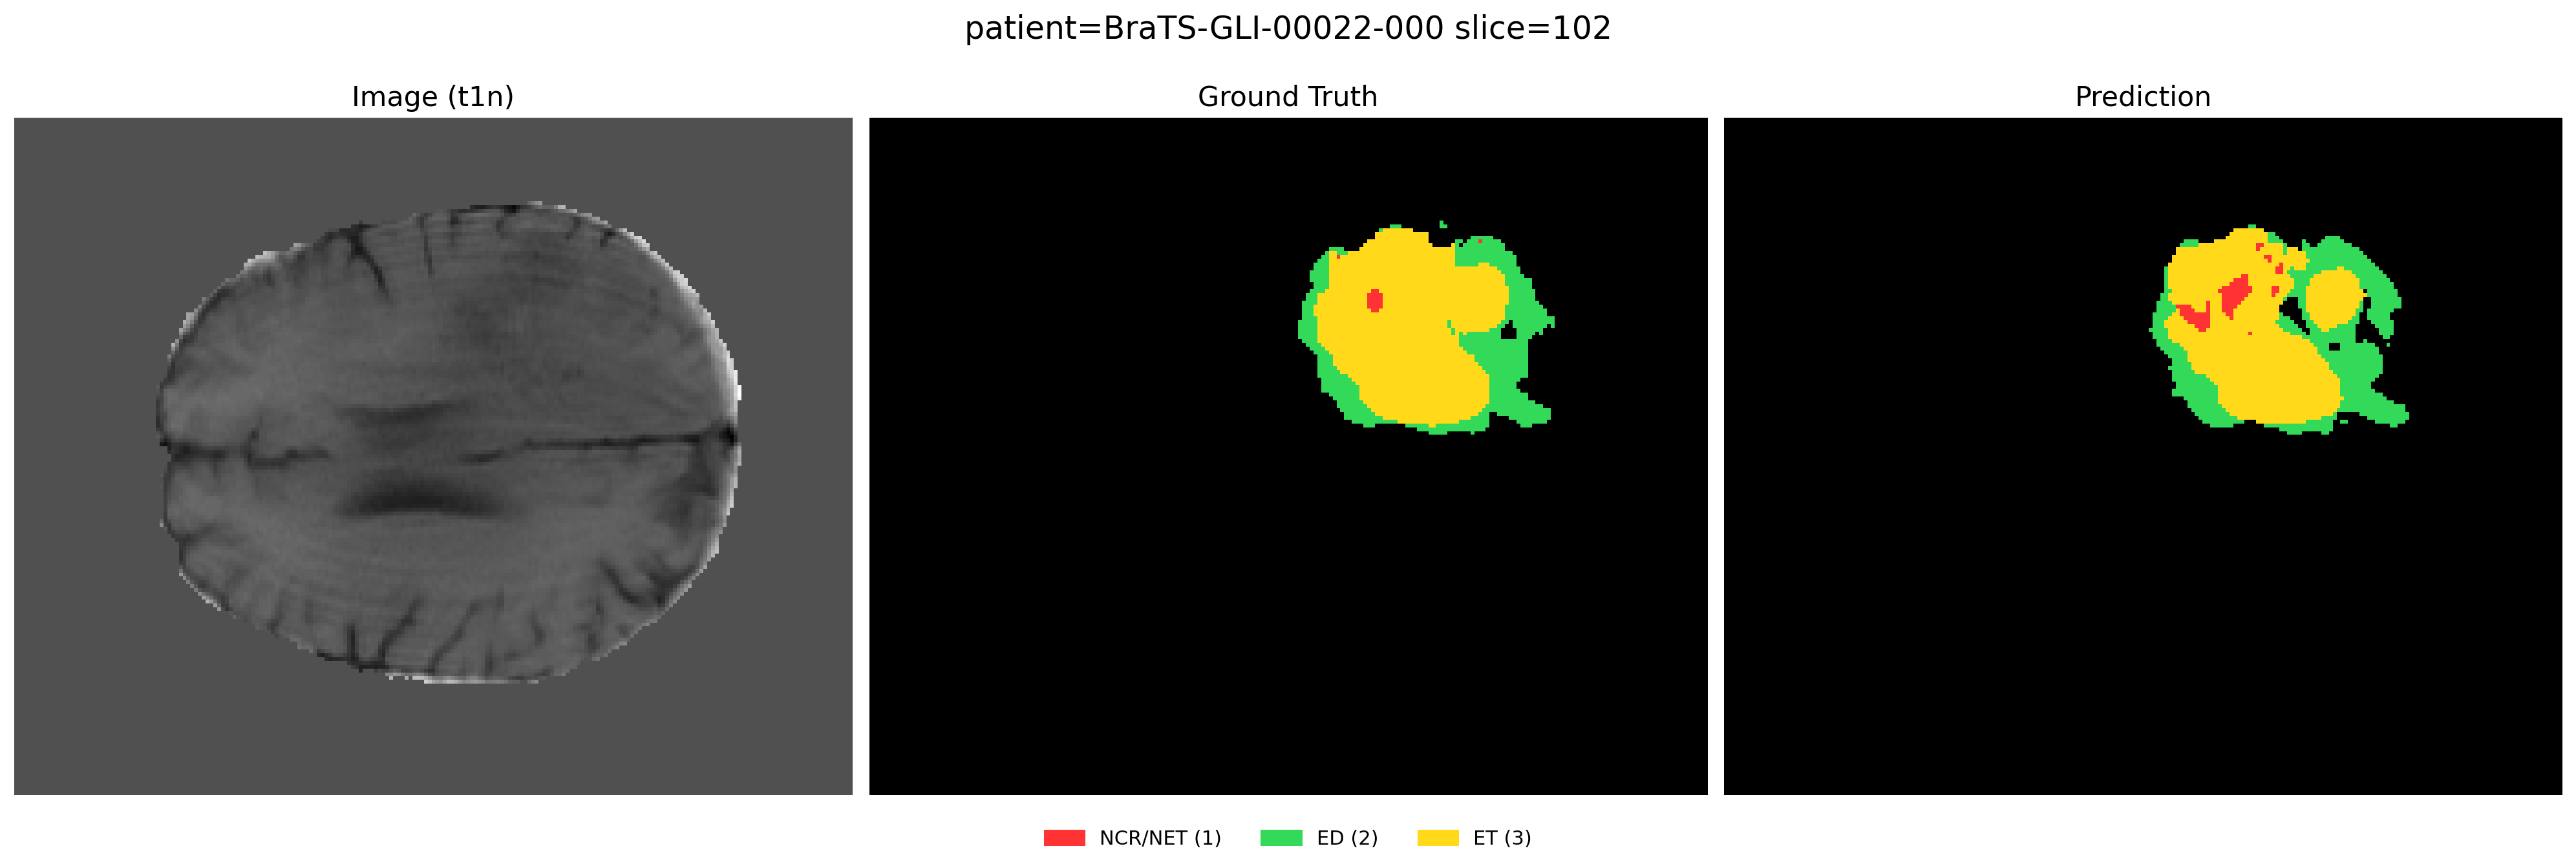
\includegraphics[width=0.58\linewidth]{../../../task2/evaluation_outputs/multiclass_all_modalities/visuals_selected_patients/BraTS-GLI-00022-000_slice_102.png}
\caption{Task 2 四模态二维模型的代表性可视化。该图用于说明预处理后多模态输入、标签和预测的基本显示方式。若最终汇报需要更突出数据处理流程，可进一步补充“原始体数据--裁剪--归一化--标签转换”的流程图。}
\end{figure}

我们还比较了 patch training 与 full-volume training。full-volume training 的结果更差，说明随机 patch 同时承担了显存控制、空间采样增强和肿瘤区域重采样三种作用。这个观察影响了后续设计：后续模型优先改进三维主干、模态融合和边界错误控制，单纯扩大输入视野并未成为主要方向。

\section{从二维 U-Net 到三维 U-Net：直接升级实验}

第一步实验尽量贴近 Task 2 的 U-Net 思路。我们将二维多模态 U-Net 改为三维版本：每个模态先经过独立 ModalityStem3D，随后在 stem-level 进行融合，再进入四级 3D encoder--decoder。该实验用于回答一个基础问题：Task 2 中有效的 U-Net 结构在三维 full-volume 协议下能否成为可靠的初始参照。

\begin{table}[H]
\centering
\caption{Task 2 四模态二维 U-Net 与 Task 3 三维 U-Net 系列的对比。Task 2 四模态模型报告了 patient-level HD95。}
\begin{tabular}{lccccc}
\toprule
模型 & WT Dice & TC Dice & ET Dice & Mean Dice & HD95 Mean \\
\midrule
Task 2 2D U-Net, all 4 modalities & 0.9257 & 0.9285 & 0.8931 & 0.9158 & 4.1394 \\
3D multimodal U-Net baseline & 0.9078 & 0.8984 & 0.8691 & 0.8918 & 4.9237 \\
3D multimodal U-Net fresh300 & 0.9173 & 0.8997 & 0.8681 & 0.8950 & 4.7443 \\
3D U-Net dual-attention fusion & 0.9108 & 0.8936 & 0.8580 & 0.8875 & 4.1125 \\
\bottomrule
\end{tabular}
\end{table}

表中可以看到，3D U-Net fresh300 的 WT Dice 达到 0.9173，说明三维 U-Net 已经能够学习主要肿瘤区域；TC 和 ET 分别为 0.8997 和 0.8681，低于 Task 2 四模态二维模型。dual-attention 版本的 HD95 Mean 降到 4.1125，但 Dice 同时下降。这个结果给出两个判断：第一，三维空间信息可以稳定建模 WT，但对 TC/ET 小区域并不天然占优；第二，简单在 stem-level 加注意力可以改善部分边界指标，整体重叠度仍受限。后续实验因此转向更强的三维空间主干和更有结构约束的模态融合。

\section{三维空间建模主干：TransBTS-lite}

3D U-Net 的结果显示，三维卷积可以利用体数据连续性，但对 TC/ET 的提升有限。下一步选择 TransBTS-lite，是因为它在三维 CNN 的局部纹理建模之外，加入 Transformer bottleneck 处理远距离空间关系。肿瘤核心、增强区域和水肿边界往往跨越多个切片；仅靠局部卷积堆叠，模型需要很深的网络才能建立这种长程依赖。TransBTS 将 deepest feature 展平成 token 后做 self-attention，正好对应课程中“利用 inter-slice spatial information”的要求。

其代码实现位于 \texttt{task3/models/transbts.py}。模型由三部分组成：
\begin{itemize}
  \item 3D CNN encoder：四级 ResConv3D，通道数为 32、64、128、256；
  \item Transformer bottleneck：将 deepest 3D feature flatten 为 token，使用 depth=2、heads=8 的 TransformerEncoder，feed-forward dimension 为 $4C$；
  \item CNN decoder：ConvTranspose3d 上采样，并与 encoder skip features 拼接恢复空间分辨率。
\end{itemize}

ResConv3D 内部包含两层 $3\times3\times3$ Conv3d、InstanceNorm3d 和 LeakyReLU(0.2)，并在通道变化时使用 $1\times1\times1$ residual projection。该结构保留了 CNN 对局部纹理的建模能力，同时用 Transformer bottleneck 补充长程空间关系。

\begin{figure}[H]
\centering
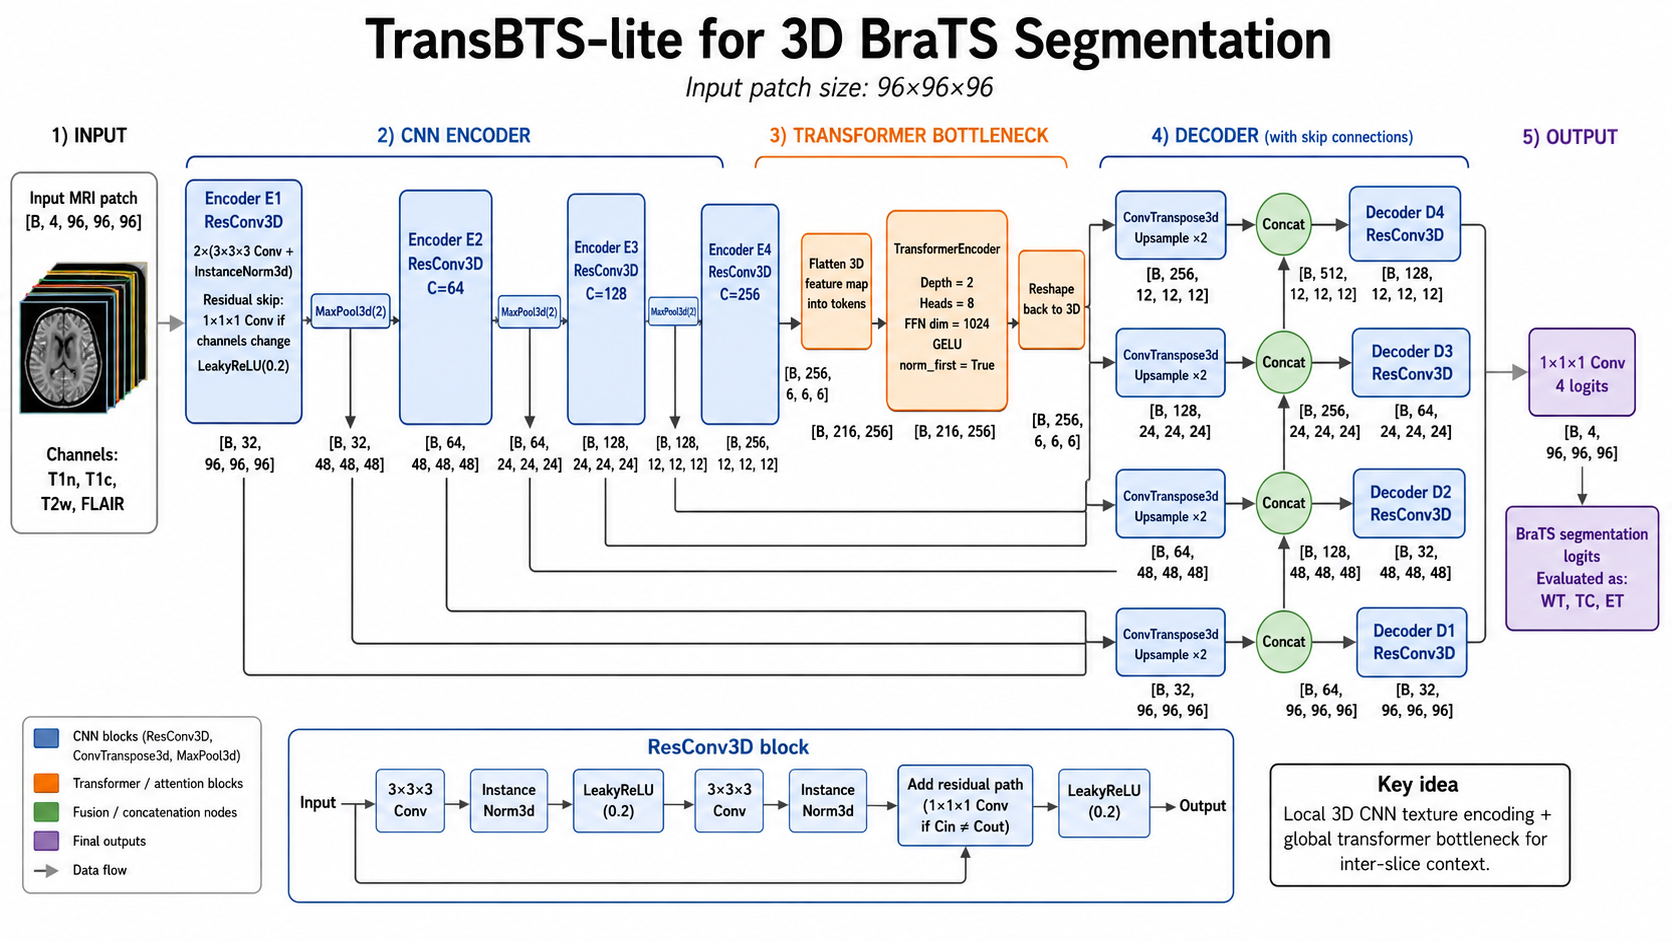
\includegraphics[width=0.92\linewidth]{../fig/model/TransBTS_lite.png}
\caption{TransBTS-lite 结构图：3D CNN encoder 负责局部纹理，Transformer bottleneck 建模全局空间关系，decoder 输出四类分割 logits。}
\end{figure}

在统一 full-volume sliding-window 测试下，TransBTS baseline 的 Mean Dice 为 0.8955，略高于 3D multimodal U-Net fresh300 的 0.8950。差异不大，但 TransBTS 的 TC Dice 从 0.8997 提高到 0.9022，ET Dice 从 0.8681 提高到 0.8711，说明 Transformer bottleneck 对较细区域有一定帮助。这个结果使 TransBTS 成为后续融合模块的主干。

\section{多模态融合探索：从输入注意力到受控特征融合}

TransBTS 仍然把四个模态作为普通输入通道处理。结合表~\ref{tab:contrast} 和 Task 2 模态实验，四个 MRI 序列的贡献明显不同：\texttt{t2f} 对 WT/TC/ET 的归一化对比度均最高，\texttt{t1c} 对 TC/ET 有明确价值，\texttt{t1n} 对肿瘤区域的对比度较弱。可视化检查中也能看到部分病灶在某些序列中更清楚。由此，后续实验围绕一个问题展开：模型能否在不同病例、不同空间位置上自适应选择模态，减少固定 concat 对弱模态和冗余模态的依赖。

\subsection{MSA-TransBTS：输入端模态-空间注意力}

MSA-TransBTS 是第一步轻量尝试。设计上尽量不改变 TransBTS 主干，只在输入端加入 ModalitySpatialAttention3D。模态注意力使用每个模态的绝对值 mean 和 max 作为全局描述，经 MLP 输出 4 个 scale；空间注意力再对通道维 mean/max 形成两个 3D map，经 $7\times7\times7$ Conv3d 得到 spatial scale。代码中 scale 写为 $2\cdot sigmoid(\cdot)$，并将最后一层初始化为 0，使初始状态接近 identity。这个初始化很重要：模型从 baseline 行为开始学习，训练初期不会突然改变输入分布。

该模块的动机可以分成两层。模态注意力处理“哪一种 MRI 序列更可信”的问题；空间注意力处理“哪些位置更像病灶”的问题。它的计算成本很小，因此适合作为第一轮探索。

\begin{figure}[H]
\centering
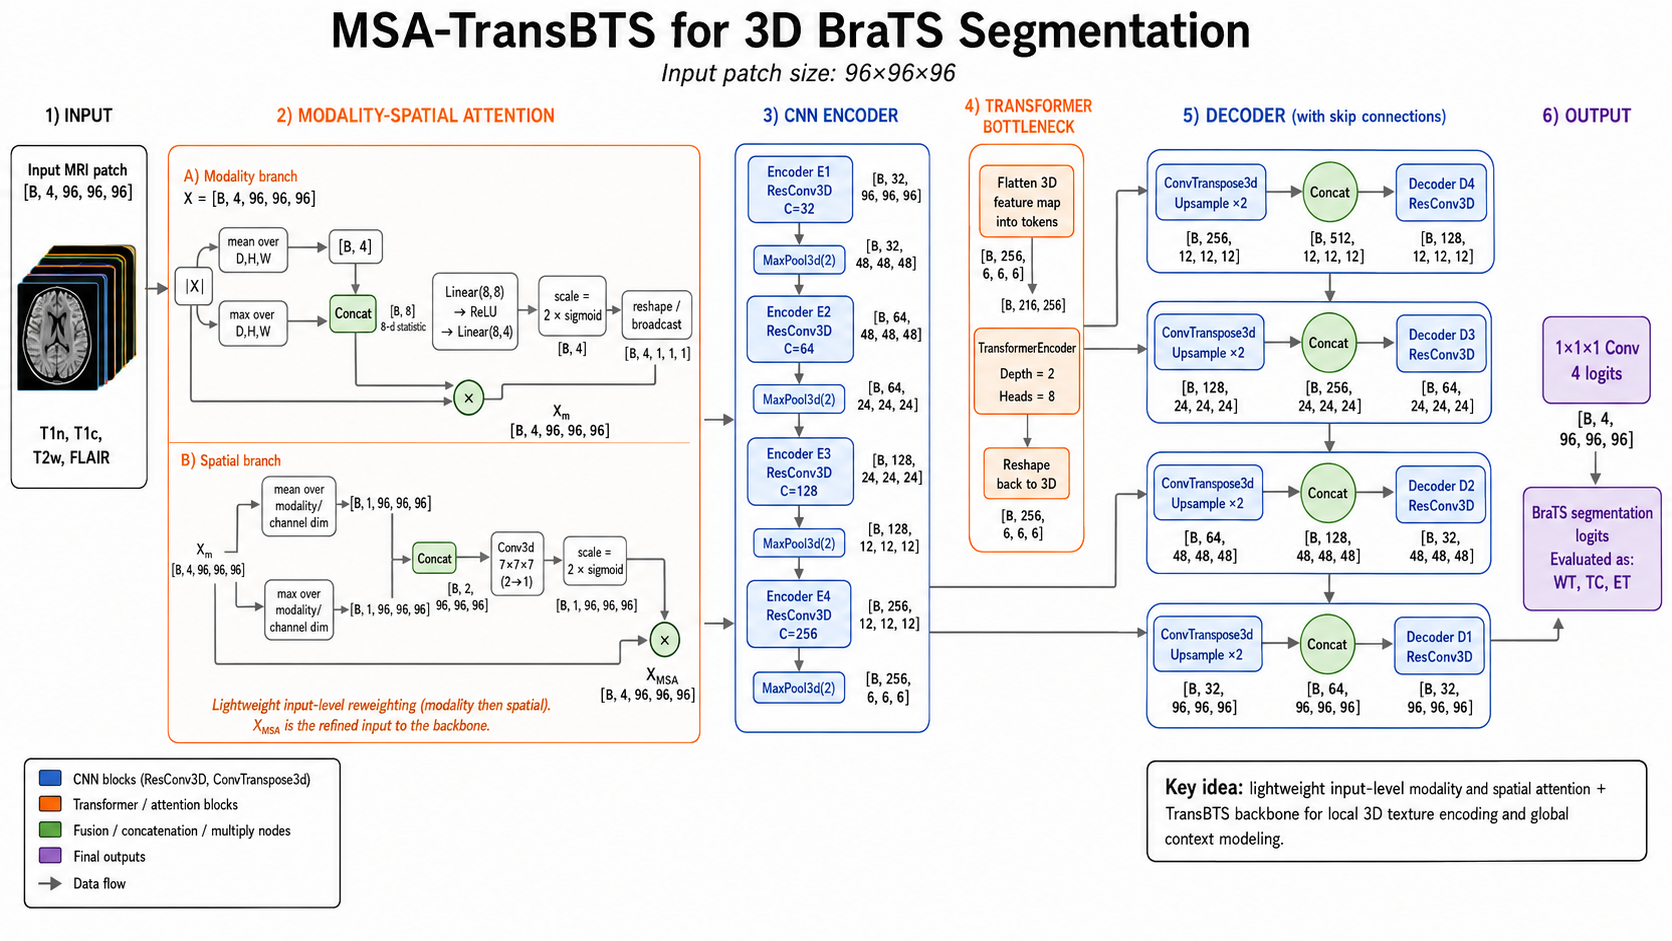
\includegraphics[width=0.92\linewidth]{../fig/model/MSA.png}
\caption{MSA-TransBTS：在主干前加入轻量模态注意力和空间注意力，尝试自动调节四模态贡献。}
\end{figure}

结果支持了部分假设，也暴露了局限。MSA 的 WT Dice 为 0.9169，高于 TransBTS baseline 的 0.9132，WT HD95 也从 4.91 降到 4.74；但 TC Dice 从 0.9022 降到 0.8938，Mean Dice 为 0.8939。这个模式说明输入端统一调节四模态对大范围 WT 有帮助，但对 TC/ET 这类小而细的区域缺少区域区分能力。下一轮实验因此把“区域”显式加入融合。

\subsection{RAM 与 RAMS：显式区域导向融合}

RAM-TransBTS 的出发点来自 MSA 的结果：如果 WT 得到改善而 TC 下降，说明一个全局模态权重很难同时服务三个临床区域。RegionAwareModalityFusion3D 因此为 WT、TC、ET 分别学习一组四模态 softmax 权重。具体实现为：根据四模态 mean/max 统计，经 MLP 输出 $3\times4$ 个权重，生成三个 region-oriented fused channels，再与原始四模态拼接为 7 通道输入 TransBTS。

RAM 的 worst-case 结果很快暴露了稳定性问题。在 BraTS-GLI-00675-001 中，RAM 的 WT 预测为空，\texttt{pred\_empty\_WT=True}，WT HD95 被记为 999.0；总体 WT HD95 均值达到 12.39。这个失败不像普通边界偏差，更接近区域响应被错误压制。RAMS-TransBTS 因此在 RAM 后加入 SharedSpatialAttention3D，用跨通道 mean/max 和 $7\times7\times7$ Conv3d 学习共享空间 scale，希望在保留区域导向融合的同时抑制不稳定空间响应。

\begin{figure}[H]
\centering
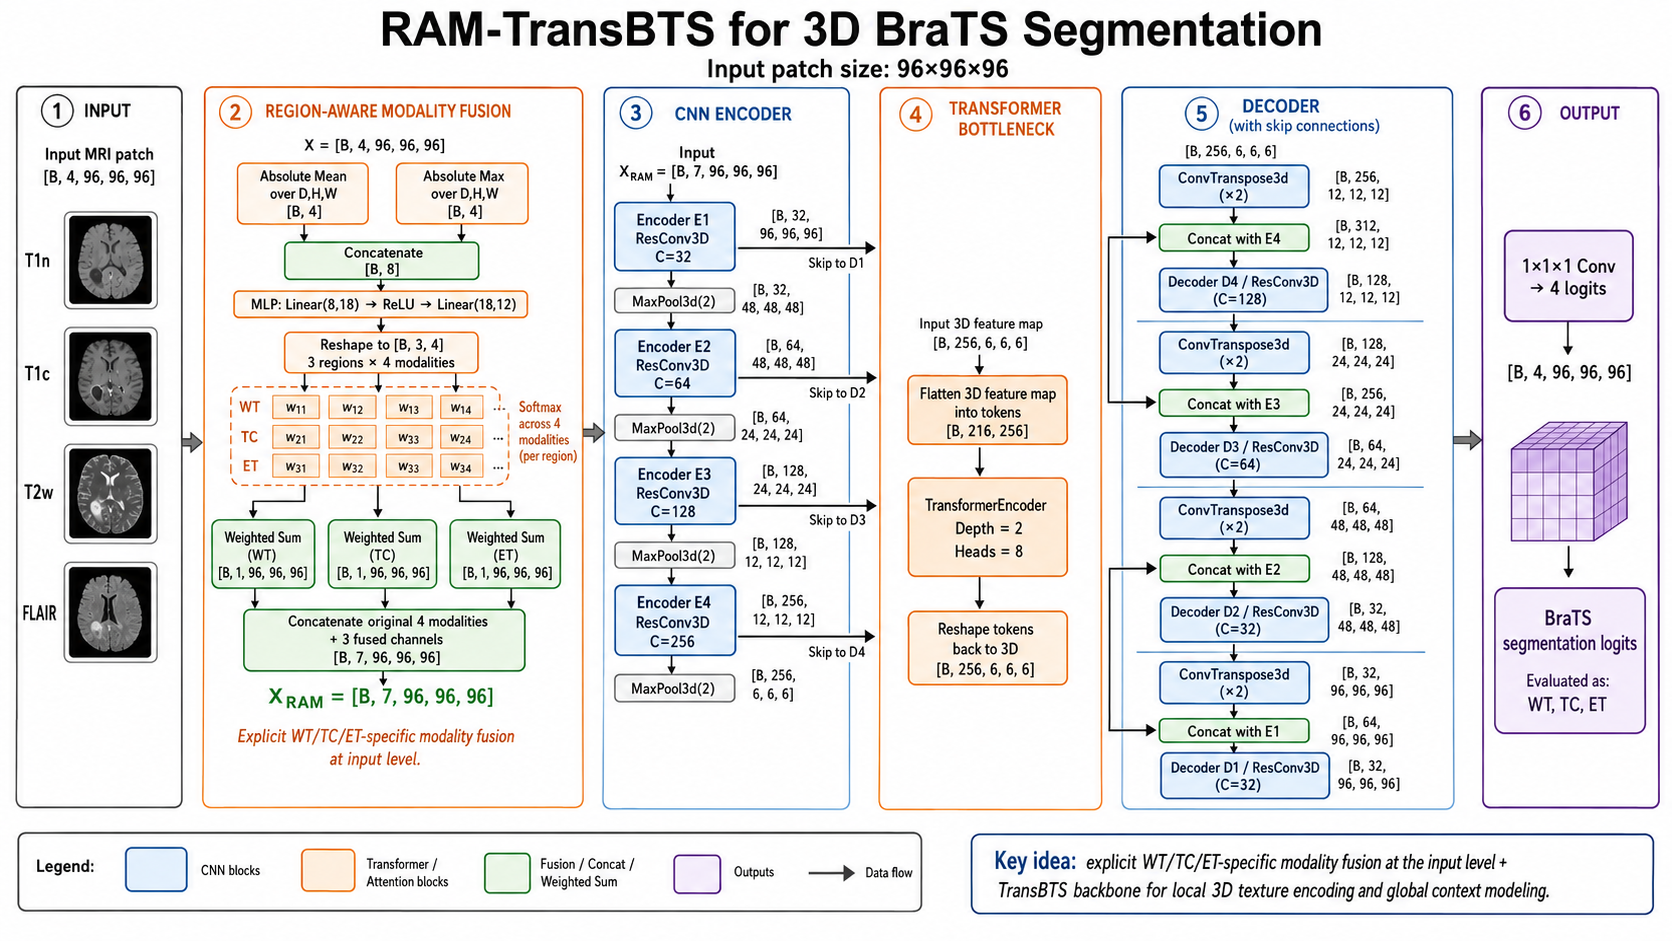
\includegraphics[width=0.48\linewidth]{../fig/model/RAM.png}
\hfill
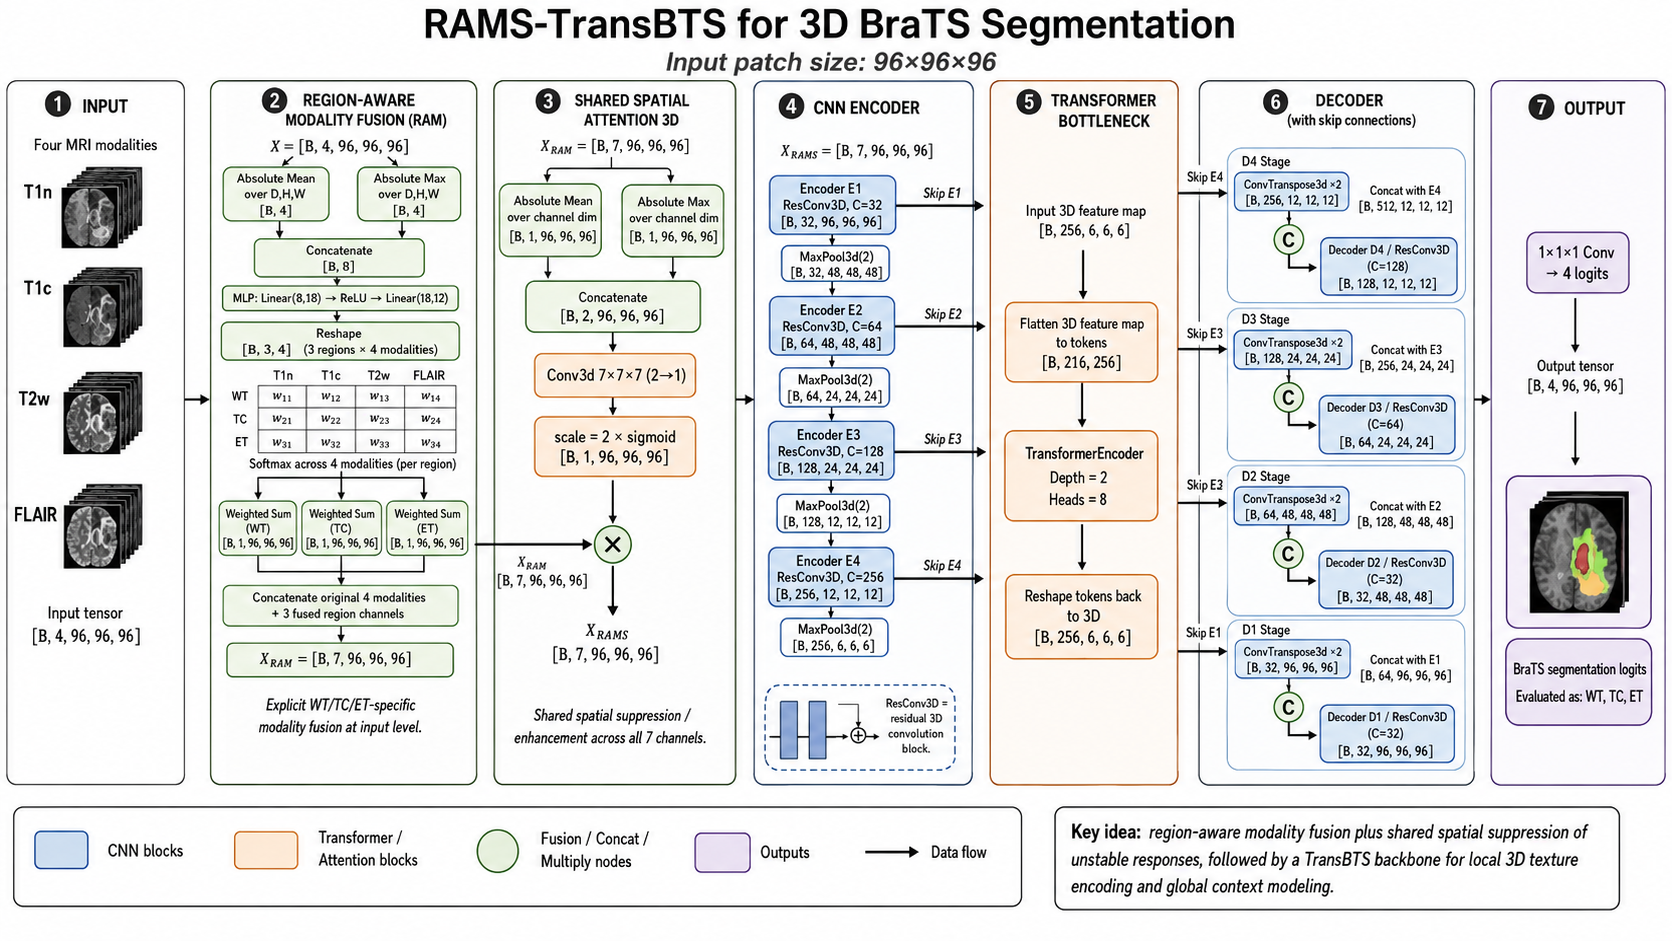
\includegraphics[width=0.48\linewidth]{../fig/model/RAMS.png}
\caption{RAM 与 RAMS：RAM 显式生成 WT/TC/ET 导向的融合通道；RAMS 在此基础上加入共享空间注意力。}
\end{figure}

RAMS 的 WT HD95 从 12.39 降到 4.62，说明共享空间注意力确实缓解了 RAM 中的极端 WT 错误；Mean Dice 仍只有 0.8924，TC/ET 收益不稳定。这个结果推动我们继续前移融合位置：只在输入层生成三个区域通道，可能不足以支持深层特征中的区域判别。

\subsection{RSF-TransBTS：区域监督特征融合的负结果}

RSF-TransBTS 的设计目标是解决 RAM/RAMS 中“融合发生得太早、区域监督太弱”的问题。它将四个模态分别送入浅层 stem，stem channel 为 4；随后 RegionSupervisedFeatureFusion3D 在 feature level 学习 WT、TC、ET 三个区域的空间变化模态权重，并为每个区域加入 auxiliary head。训练中加入 auxiliary loss（权重 0.3）和 nested constraint（权重 0.05），采样策略也从纯随机改为 region-balanced sampling：WT 0.35、TC 0.25、ET 0.25、random 0.15。

这一步的假设很直接：TC/ET 体素少，随机 patch 中出现频率低；通过区域平衡采样和辅助监督，模型应当更频繁看到小区域，并在浅层特征上学习区域相关的模态组合。

\begin{figure}[H]
\centering
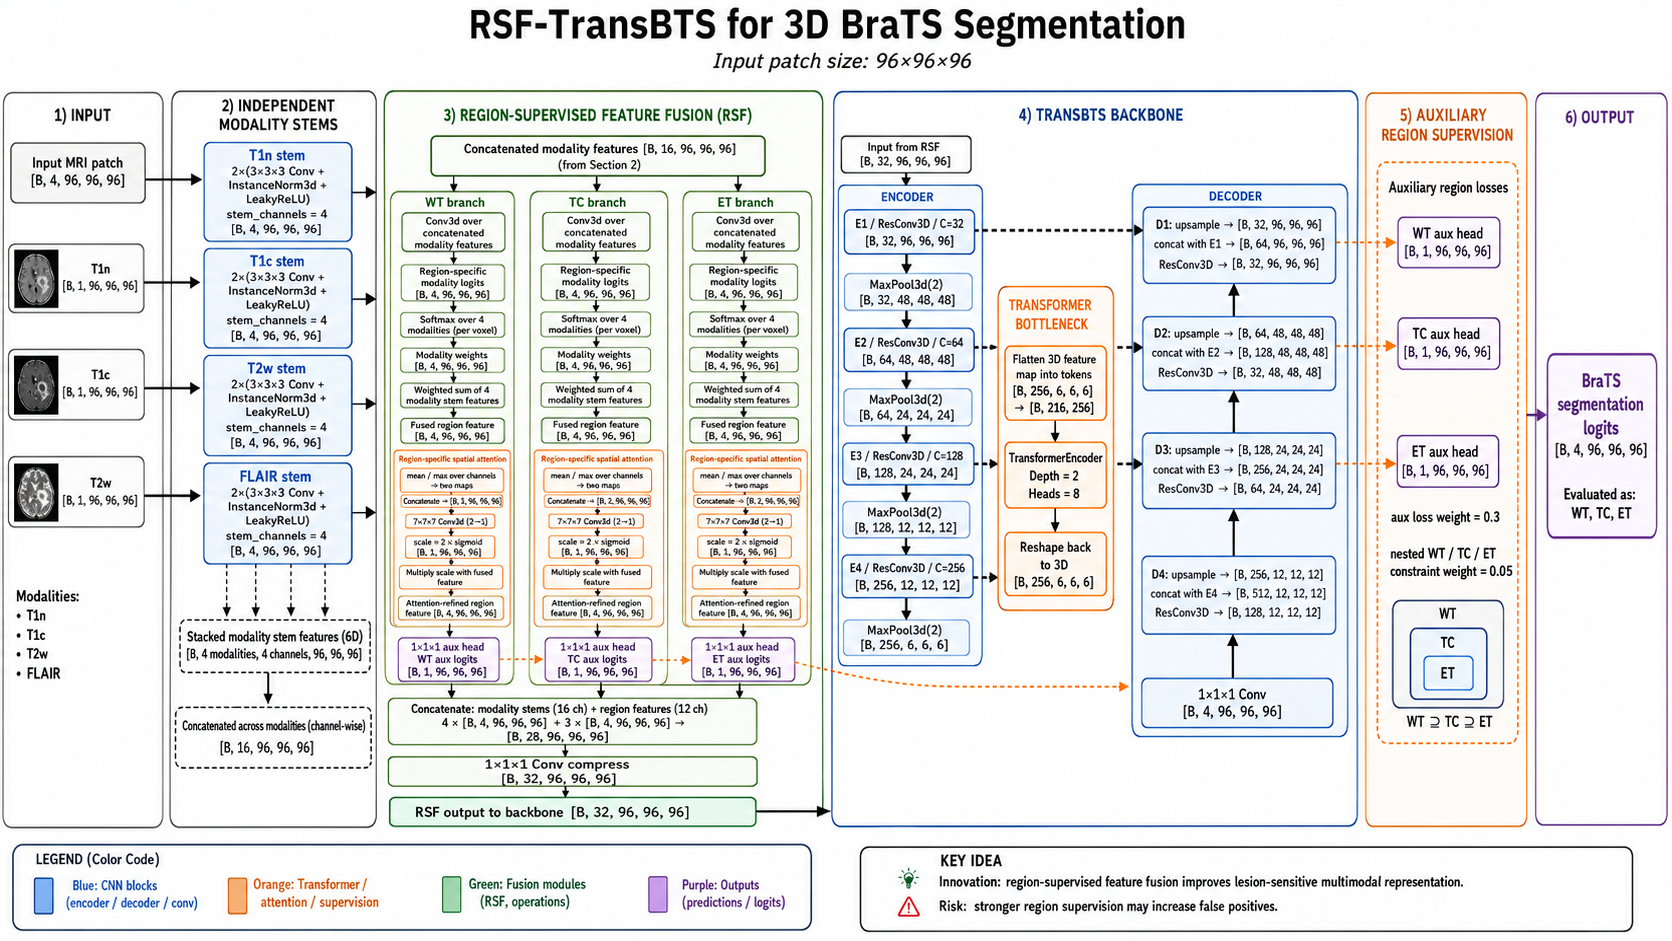
\includegraphics[width=0.92\linewidth]{../fig/model/rsf.png}
\caption{RSF-TransBTS：区域监督的 feature-level 多模态融合。该方向提升了病灶响应敏感性，但测试泛化不稳定。}
\end{figure}

测试结果与设计初衷出现明显偏差。RSF 的 Mean Dice 只有 0.8805，WT/TC/ET HD95 分别为 10.10、5.96、5.81。worst cases 中，BraTS-GLI-00321-000 的 WT/TC/ET HD95 分别达到 80.73、109.24、111.77；BraTS-GLI-00733-001 的 WT HD95 为 90.72。图~\ref{fig:rsf_badcase} 展示了这种远端假阳性和不连续预测。由此得到的经验是：区域监督和病灶采样提高了敏感性，同时也放大了对疑似病灶的响应。后续 TAF 设计减少对区域辅助头的依赖，优先约束融合的数值形式。

\begin{figure}[H]
\centering
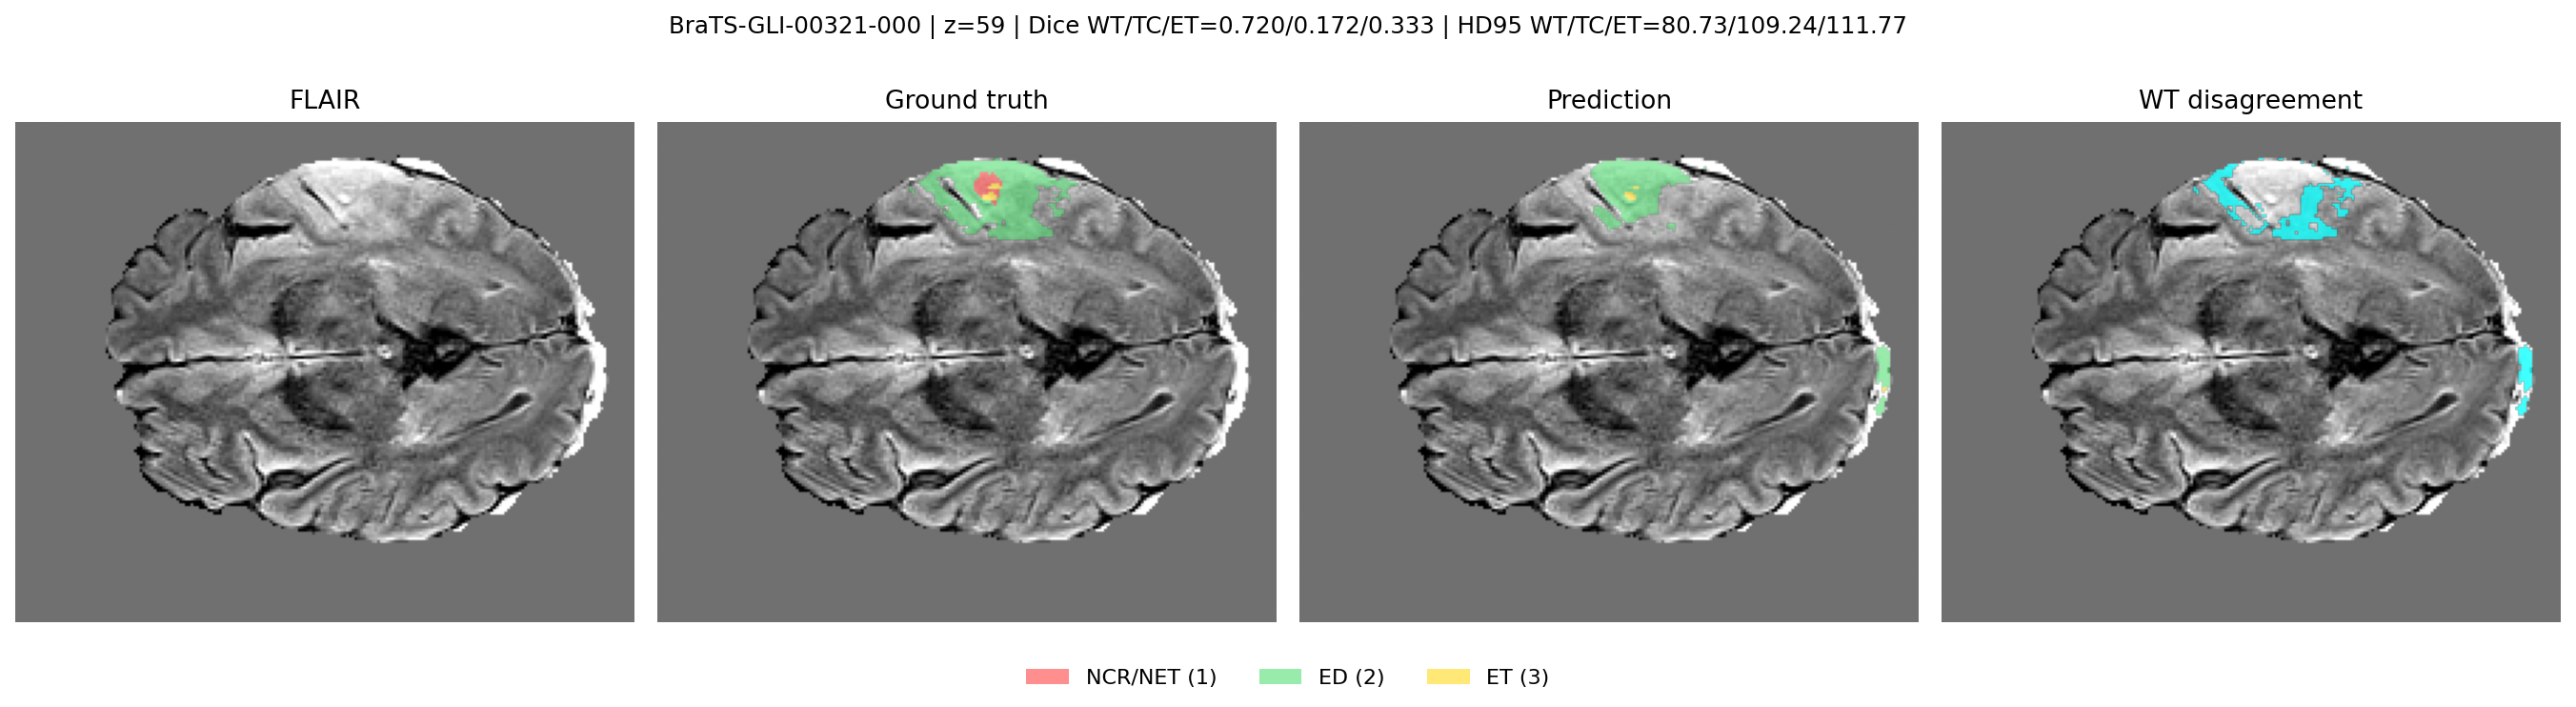
\includegraphics[width=0.48\linewidth]{../../outputs/rsf_transbts_regionfusion_rerun/analysis/worst_case_figures_test/BraTS-GLI-00321-000.png}
\hfill
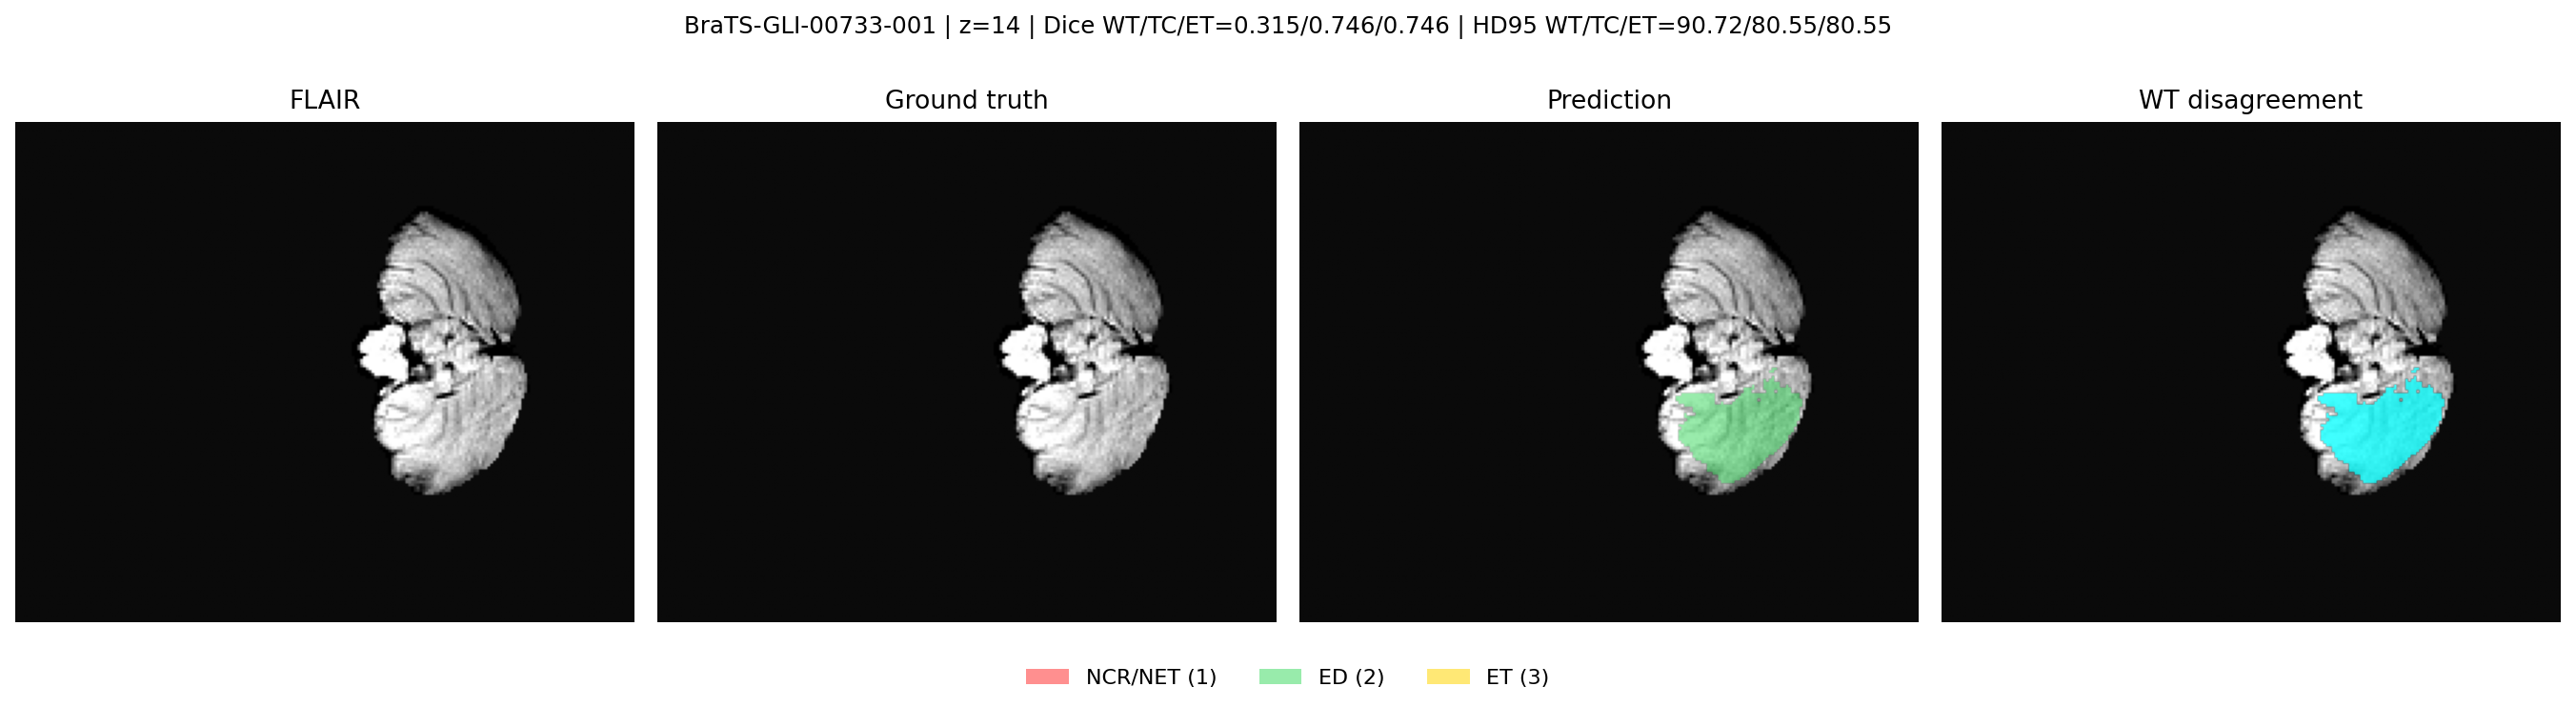
\includegraphics[width=0.48\linewidth]{../../outputs/rsf_transbts_regionfusion_rerun/analysis/worst_case_figures_test/BraTS-GLI-00733-001.png}
\caption{RSF-TransBTS 的代表性失败病例。强区域监督提高了病灶响应，但在部分病例中产生远端假阳性和 HD95 tail error。}
\label{fig:rsf_badcase}
\end{figure}

\section{最终方案：TAF-TransBTS A3}

前面几轮实验形成了一个较清晰的约束：MSA 表明模态注意力有价值，RAM/RAMS 表明区域导向融合需要控制空间稳定性，RSF 表明过强区域监督会带来远端假阳性。TAF-TransBTS A3 在这个基础上重新组织融合方式：保留四模态独立表达，并用 softmax 约束融合权重，使融合结果保持为模态特征的凸组合。

TAF-TransBTS A3 的结构如下：
\begin{itemize}
  \item 四个模态分别进入独立 ModalityEncoder3D，base channel 为 24，四级 encoder 通道为 24、48、96、192；
  \item 每一级 skip feature 均通过 DualAttentionFusion3D 融合；
  \item DualAttentionFusion3D 同时包含 modality attention 和 spatial attention：前者根据每个模态特征的 mean/max 统计，经 MLP 得到四模态 softmax 权重；后者将四模态 feature concat 后经 $3\times3\times3$ Conv3d 得到空间位置相关的四模态 softmax 权重；
  \item 两条路径的输出取平均，形成融合特征；
  \item deepest feature 经同样的 fusion 后进入 Transformer bottleneck，depth=2，heads=8；
  \item A3 配置中关闭 correlation loss，\texttt{correlation\_enabled=false}，\texttt{loss\_correlation\_weight=0}。因此，当前结果只评价独立模态 encoder 与 softmax-controlled dual attention fusion。
\end{itemize}

与 RSF 中的 sigmoid scale 相比，softmax 权重不会同时放大所有模态响应。每个位置的输出由四个模态竞争得到，这与前面观察到的“某些病例只在部分序列中表现清楚”相吻合，也能限制远端假阳性在深层特征中被持续增强。

\begin{figure}[H]
\centering
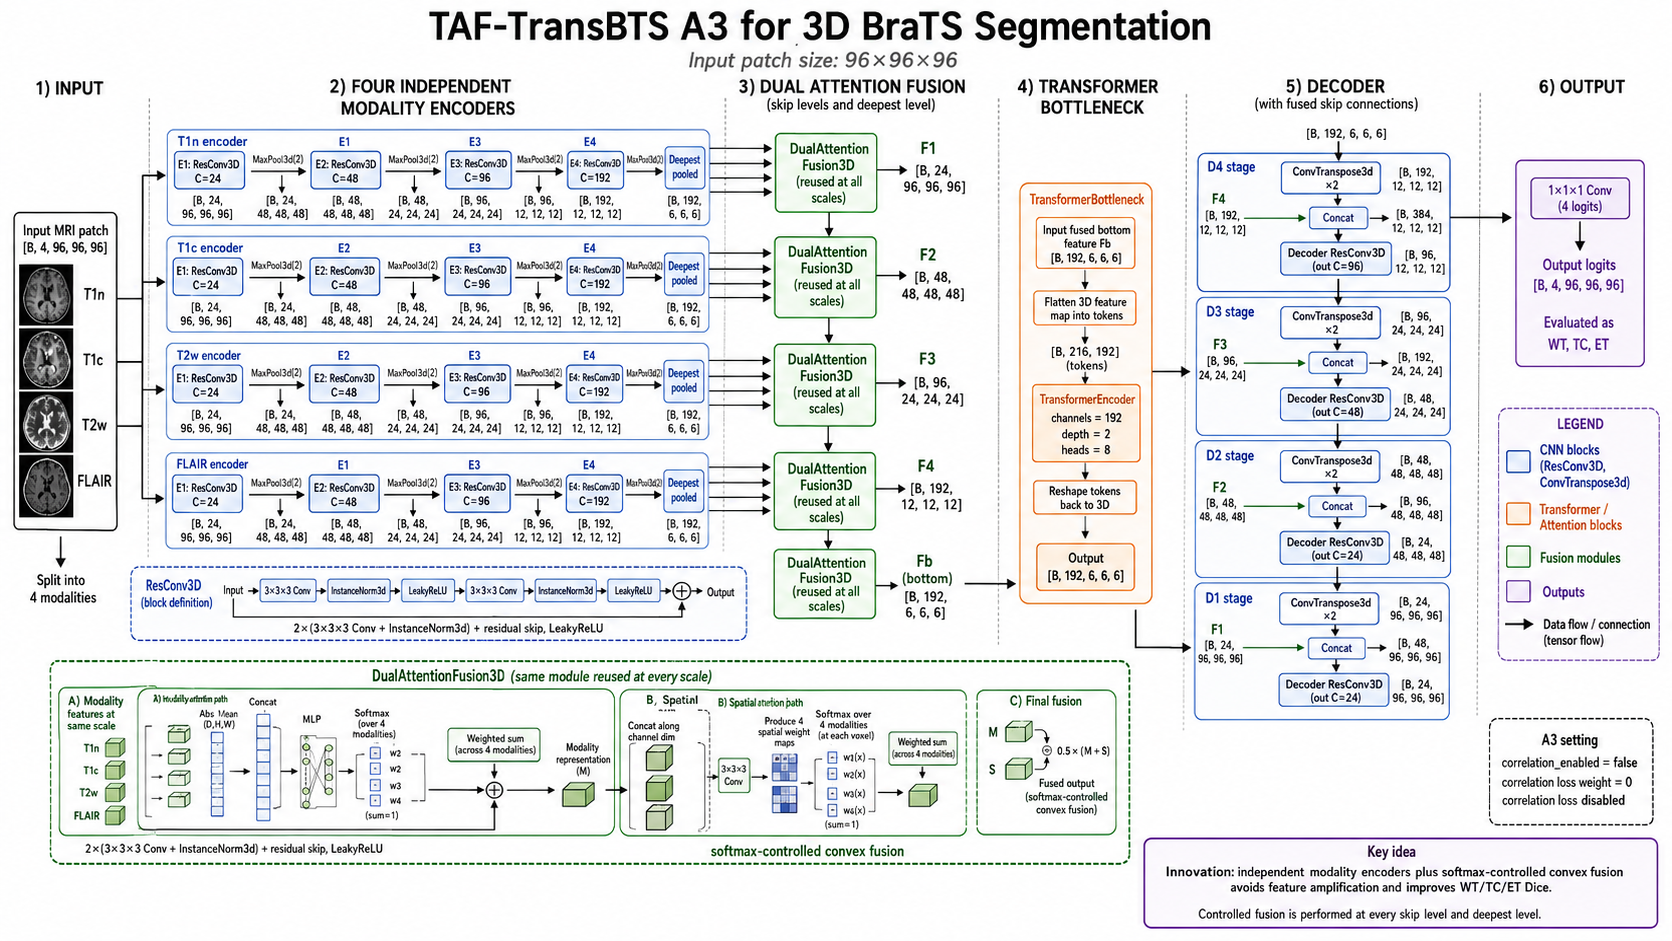
\includegraphics[width=0.95\linewidth]{../fig/model/taf_transbts_a3.png}
\caption{TAF-TransBTS A3：四模态独立编码，并在多尺度 skip 与 deepest feature 上进行 softmax-controlled dual attention fusion。}
\end{figure}

\section{实验结果与 HD95 分析}

\subsection{全部主要 Task 3 模型结果}

\begin{table}[H]
\centering
\caption{Task 3 主要模型在 test split 上的 full-volume sliding-window 结果。Dice 越高越好，HD95 越低越好。}
\resizebox{\linewidth}{!}{
\begin{tabular}{lrrrrrrr}
\toprule
模型 & WT Dice & TC Dice & ET Dice & Mean Dice & WT HD95 & TC HD95 & ET HD95 \\
\midrule
Attention U-Net 3D & 0.9006 & 0.8930 & 0.8628 & 0.8854 & 6.12 & 3.35 & 2.76 \\
SwinUNETR v2 & 0.9089 & 0.8952 & 0.8598 & 0.8879 & 5.91 & 5.85 & 5.35 \\
Multimodal U-Net attention & 0.9122 & 0.8886 & 0.8655 & 0.8888 & 6.44 & 4.82 & 4.07 \\
3D multimodal U-Net fresh300 & 0.9173 & 0.8997 & 0.8681 & 0.8950 & 6.01 & 4.22 & 4.00 \\
TransBTS baseline & 0.9132 & 0.9022 & 0.8711 & 0.8955 & 4.91 & 3.26 & 3.62 \\
MSA-TransBTS & 0.9169 & 0.8938 & 0.8709 & 0.8939 & 4.74 & 3.84 & 3.00 \\
RAM-TransBTS & 0.9105 & 0.8982 & 0.8677 & 0.8921 & 12.39 & 3.53 & 2.96 \\
RAMS-TransBTS & 0.9148 & 0.8969 & 0.8654 & 0.8924 & 4.62 & 3.41 & 3.33 \\
RSF-TransBTS & 0.8893 & 0.8912 & 0.8610 & 0.8805 & 10.10 & 5.96 & 5.81 \\
Staged TAF-TransBTS A3 & 0.9160 & 0.9087 & 0.8774 & 0.9007 & 5.41 & 3.73 & 3.49 \\
Fresh TransBTS control & 0.9149 & 0.9063 & 0.8724 & 0.8979 & 12.40 & 3.06 & 2.80 \\
\textbf{Fresh TAF-TransBTS A3} & \textbf{0.9190} & \textbf{0.9106} & 0.8745 & \textbf{0.9014} & 5.71 & \textbf{2.94} & 3.46 \\
\bottomrule
\end{tabular}
}
\end{table}

Attention U-Net 和 SwinUNETR 作为课程要求中的 advanced baselines 保留在表格中，但不作为主线展开。它们说明我们确实比较了注意力 U-Net 和 transformer-style 3D architecture。相比之下，\texttt{multimodal\_unet\_attention} 与 3D multimodal U-Net 系列更接近重复验证，用于说明 naive 多模态 U-Net 和简单 stem-level attention 不足以突破，因此不放入主要叙事章节。

\subsection{Fresh control：最干净的结构证据}

为了排除 staged fine-tuning 或 warm-start 带来的混淆，我们进行了 Fresh TransBTS control 与 Fresh TAF-TransBTS A3 的同协议对照。两者均从随机初始化开始，使用相同 split、相同增强、相同 $96^3$ patch、相同 BF16 mixed precision、相同 Adam 与 plateau scheduler，并每 10 epoch 进行 full-volume validation。

\begin{table}[H]
\centering
\caption{Fresh TAF-TransBTS A3 与 Fresh TransBTS 的公平对照。}
\begin{tabular}{lrrr}
\toprule
指标 & Fresh TransBTS & Fresh TAF A3 & A3 - TransBTS \\
\midrule
Full-val Mean Dice & 0.9328 & 0.9341 & +0.0013 \\
WT Dice & 0.9149 & 0.9190 & +0.0041 \\
TC Dice & 0.9063 & 0.9106 & +0.0043 \\
ET Dice & 0.8724 & 0.8745 & +0.0021 \\
Mean Dice & 0.8979 & 0.9014 & +0.0035 \\
WT HD95 & 12.40 & 5.71 & -6.69 \\
TC HD95 & 3.06 & 2.94 & -0.11 \\
ET HD95 & 2.80 & 3.46 & +0.66 \\
\bottomrule
\end{tabular}
\end{table}

这组结果是当前最可靠的结构证据：TAF A3 在 WT、TC、ET 三个 Dice 上均超过同协议 TransBTS，并将 Mean Dice 提升到 0.9014。HD95 方面，Fresh TransBTS 的 WT HD95 为 12.40，Fresh A3 降到 5.71；TC HD95 也从 3.06 降到 2.94。ET HD95 从 2.80 升到 3.46，提示增强肿瘤边界仍然是未解决的细粒度问题。

与 Task 2 四模态二维 U-Net 相比，Fresh A3 的 Mean Dice 较低（0.9014 vs. 0.9158），WT HD95 略高（5.71 vs. 5.03），TC HD95 更低（2.94 vs. 3.95），ET HD95 接近（3.46 vs. 3.43）。这些数字显示二维模型在 Dice 上仍有优势；Task 3 的主要增量集中在三维全体积协议下验证空间建模和多模态受控融合，尤其是在同协议 3D baseline 上改善 WT/TC 的 HD95 tail risk。

\section{Bad-case 与优秀 case 分析}

课程要求对 worst-performing cases 进行分析，判断失败是否来自低对比、小病灶或伪影。我们基于 staged TAF-TransBTS A3 的 per-case 结果进行了描述性分析。该 checkpoint 在 127 个测试病例上没有出现 WT、TC 或 ET 的 infinite HD95，说明不存在系统性完全崩溃。

\begin{table}[H]
\centering
\caption{TAF-TransBTS A3 的五个最低 Mean-Dice 病例及主要失败模式。}
\begin{tabular}{lrrrrp{6.3cm}}
\toprule
病例 & WT & TC & ET & Mean & 主要失败模式 \\
\midrule
BraTS-GLI-00621-000 & 0.752 & 0.141 & 0.141 & 0.345 & 薄而复杂的增强区域，TC/ET 严重 under-segmentation。 \\
BraTS-GLI-00331-000 & 0.443 & 0.214 & 0.438 & 0.365 & 低对比 diffuse WT，预测碎片化，并有远端假阳性。 \\
BraTS-GLI-00525-001 & 0.975 & 0.387 & 0.098 & 0.486 & WT 很好，但薄 enhancing rim 和 TC/ET 明显漏分。 \\
BraTS-GLI-00021-000 & 0.744 & 0.364 & 0.424 & 0.511 & 水肿边界弥散且不规则，预测组件碎片化。 \\
BraTS-GLI-00684-000 & 0.760 & 0.465 & 0.465 & 0.563 & 小 peripheral lesion，TC/ET 证据不足。 \\
\bottomrule
\end{tabular}
\end{table}

\begin{figure}[H]
\centering
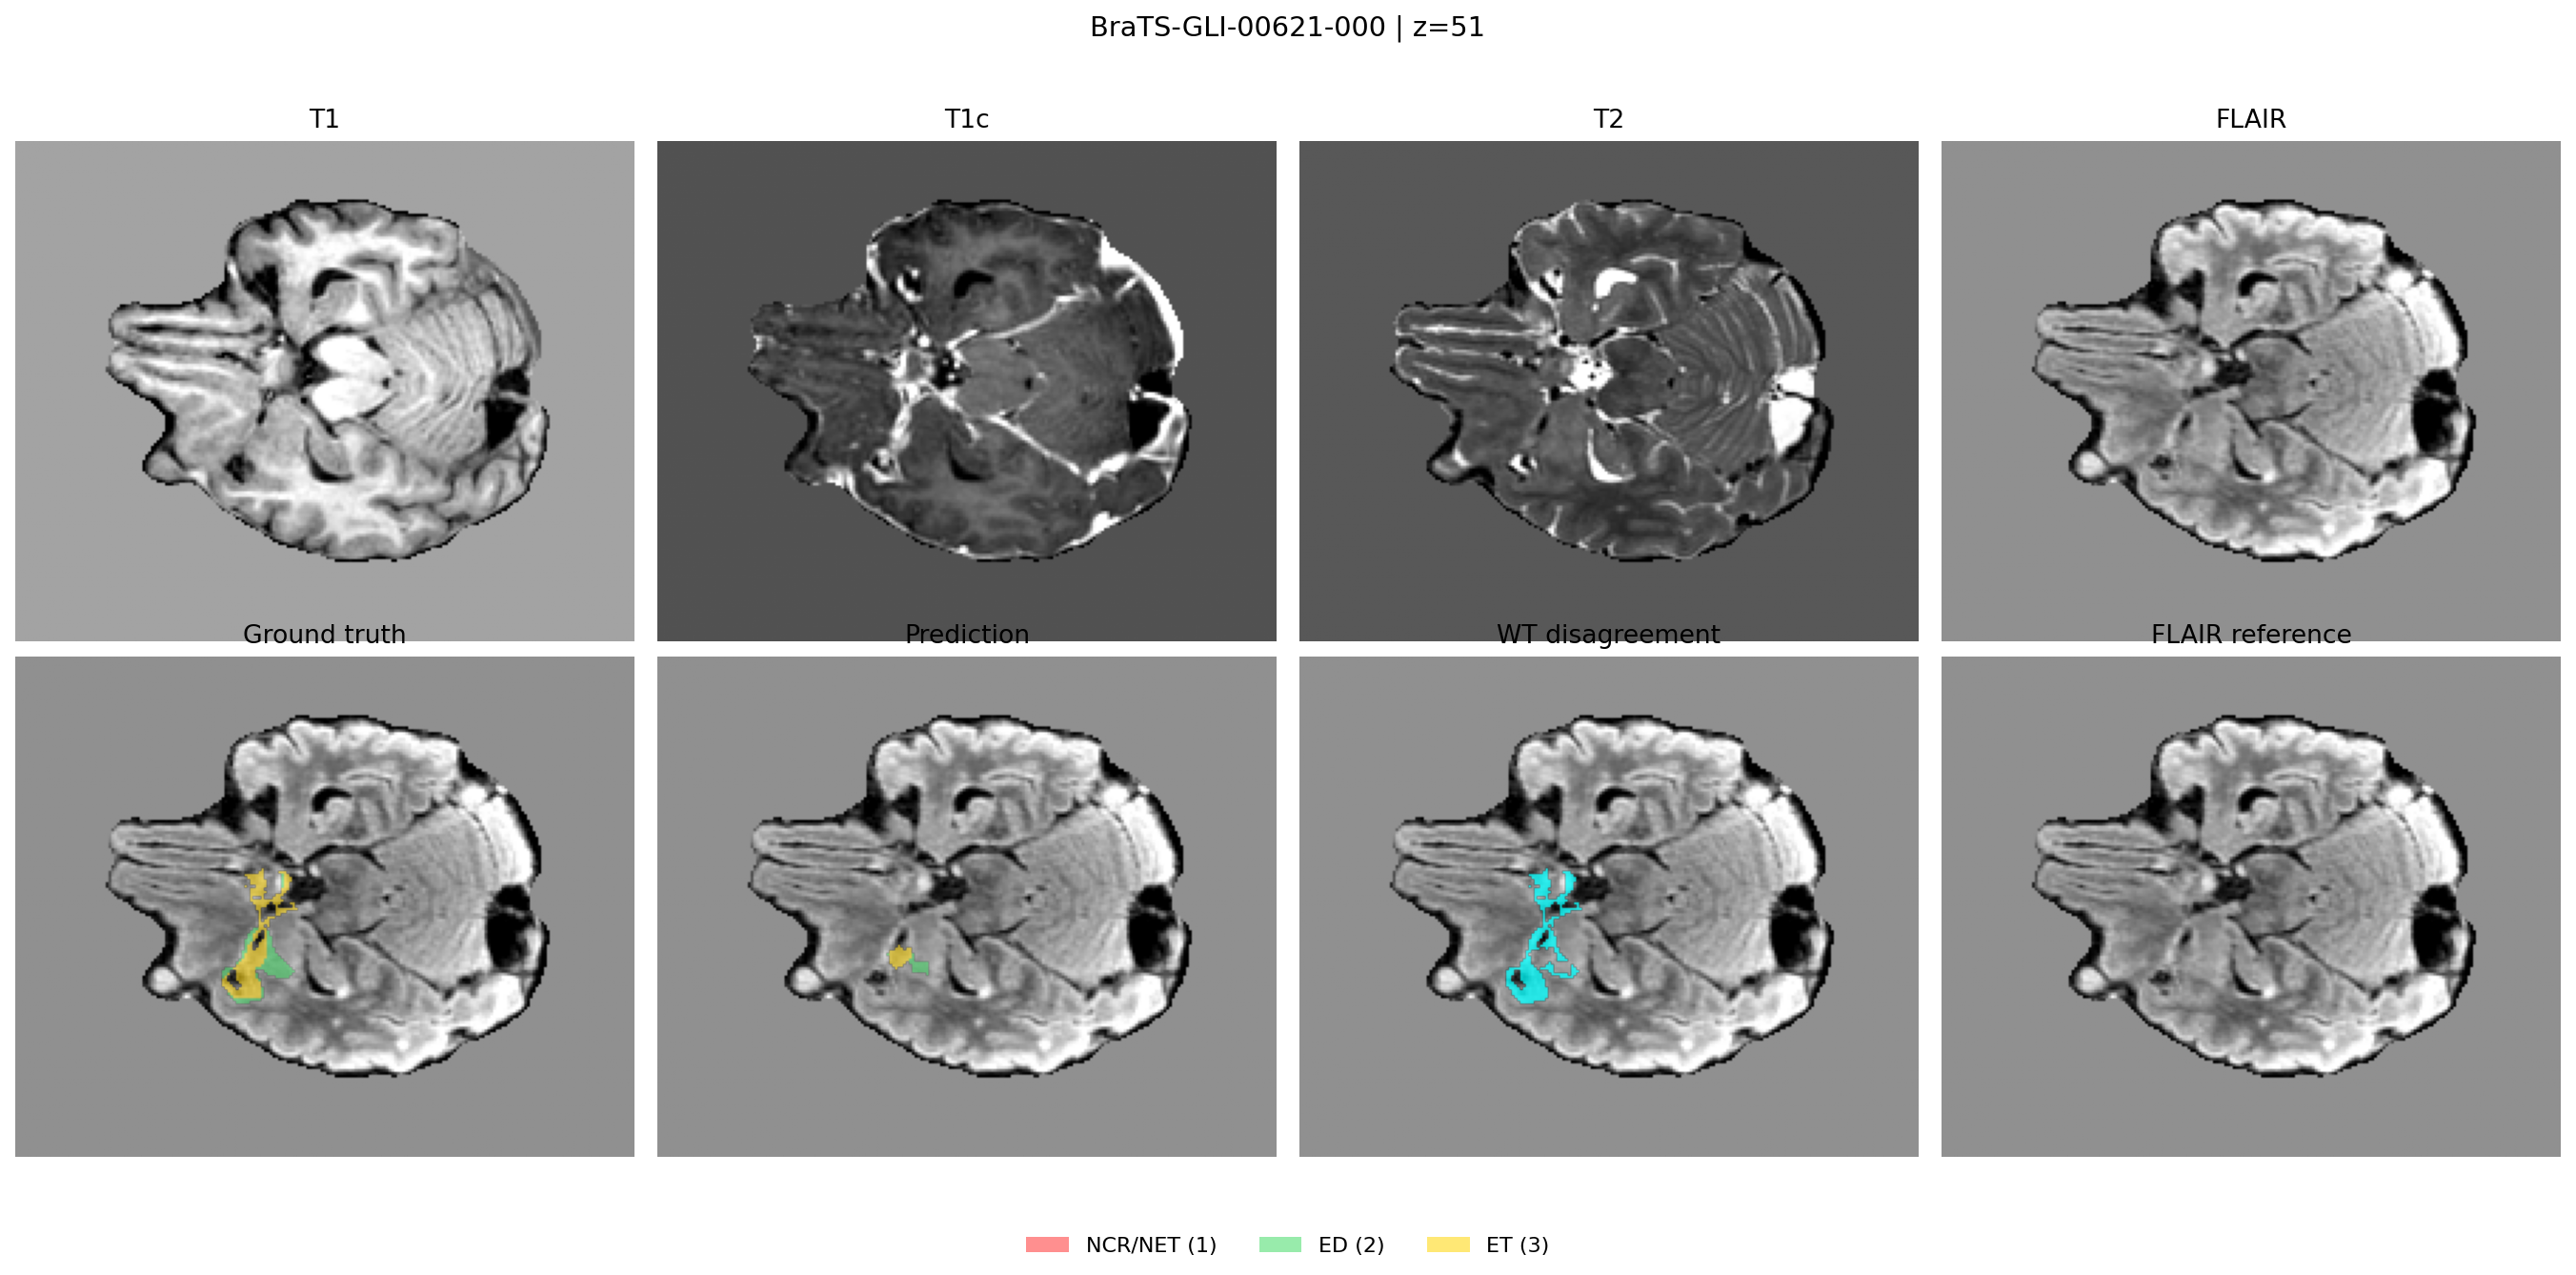
\includegraphics[width=0.48\linewidth]{../../outputs/taf_transbts_cluster_a3_finetune_resume_mmap/analysis/multimodal_badcase_figures_test/BraTS-GLI-00621-000.png}
\hfill
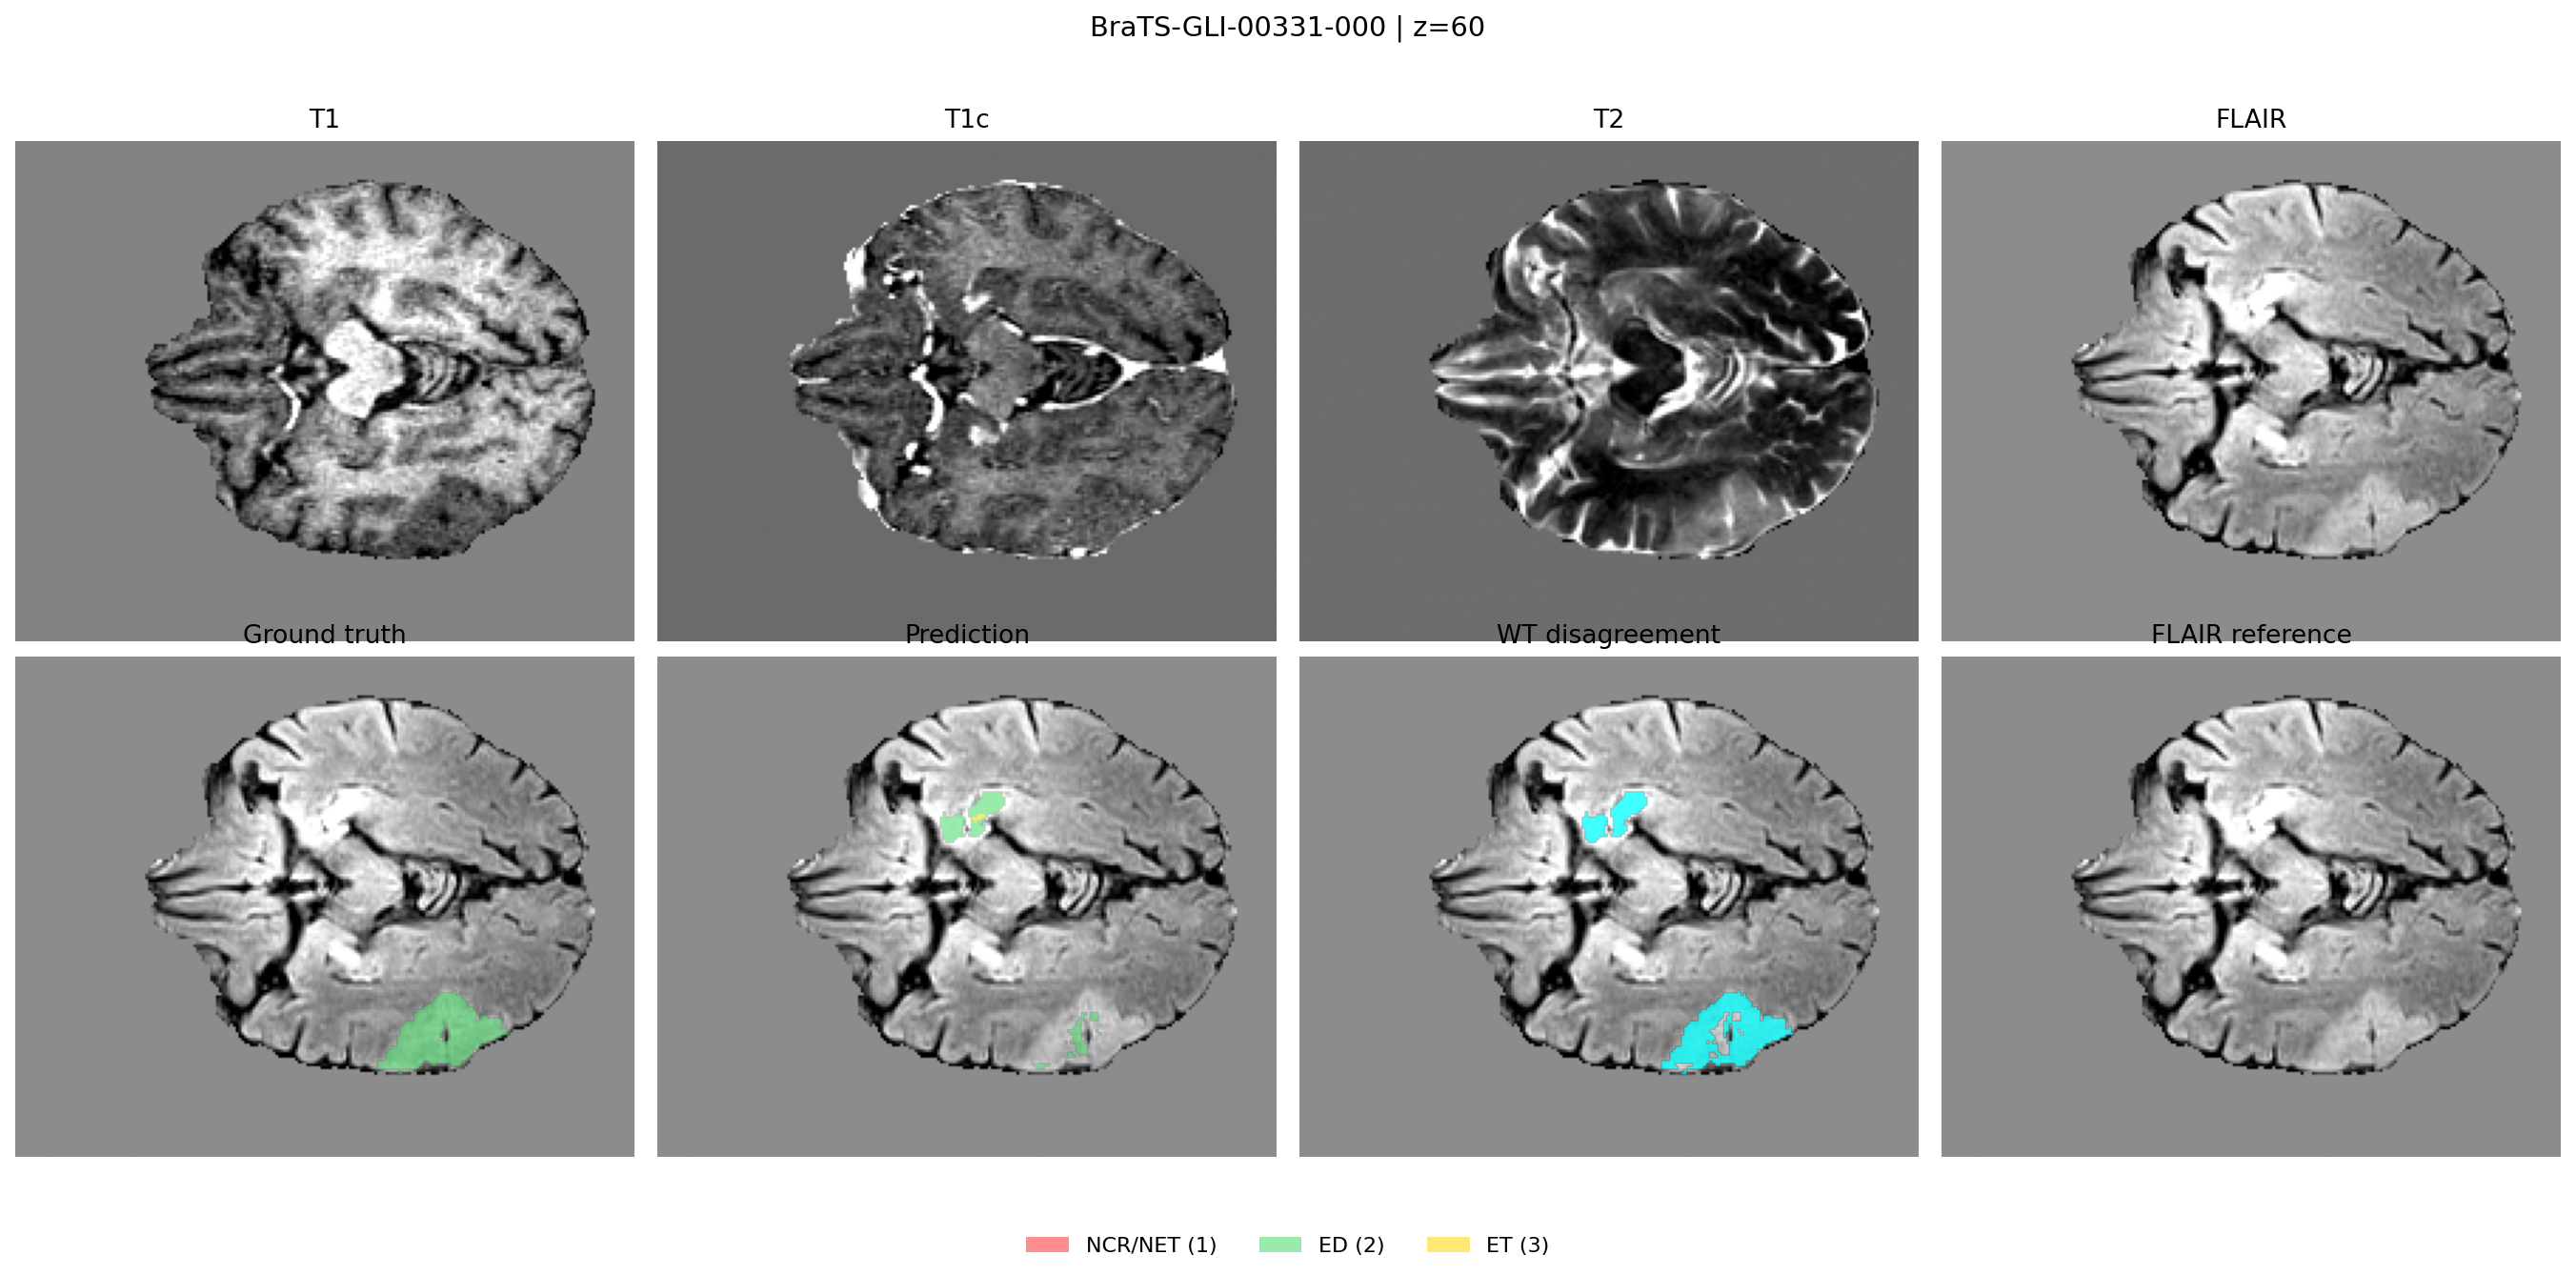
\includegraphics[width=0.48\linewidth]{../../outputs/taf_transbts_cluster_a3_finetune_resume_mmap/analysis/multimodal_badcase_figures_test/BraTS-GLI-00331-000.png}
\caption{代表性 bad cases：左侧为薄 TC/ET 漏分，右侧为低对比 WT 与远端假阳性。}
\end{figure}

\begin{figure}[H]
\centering
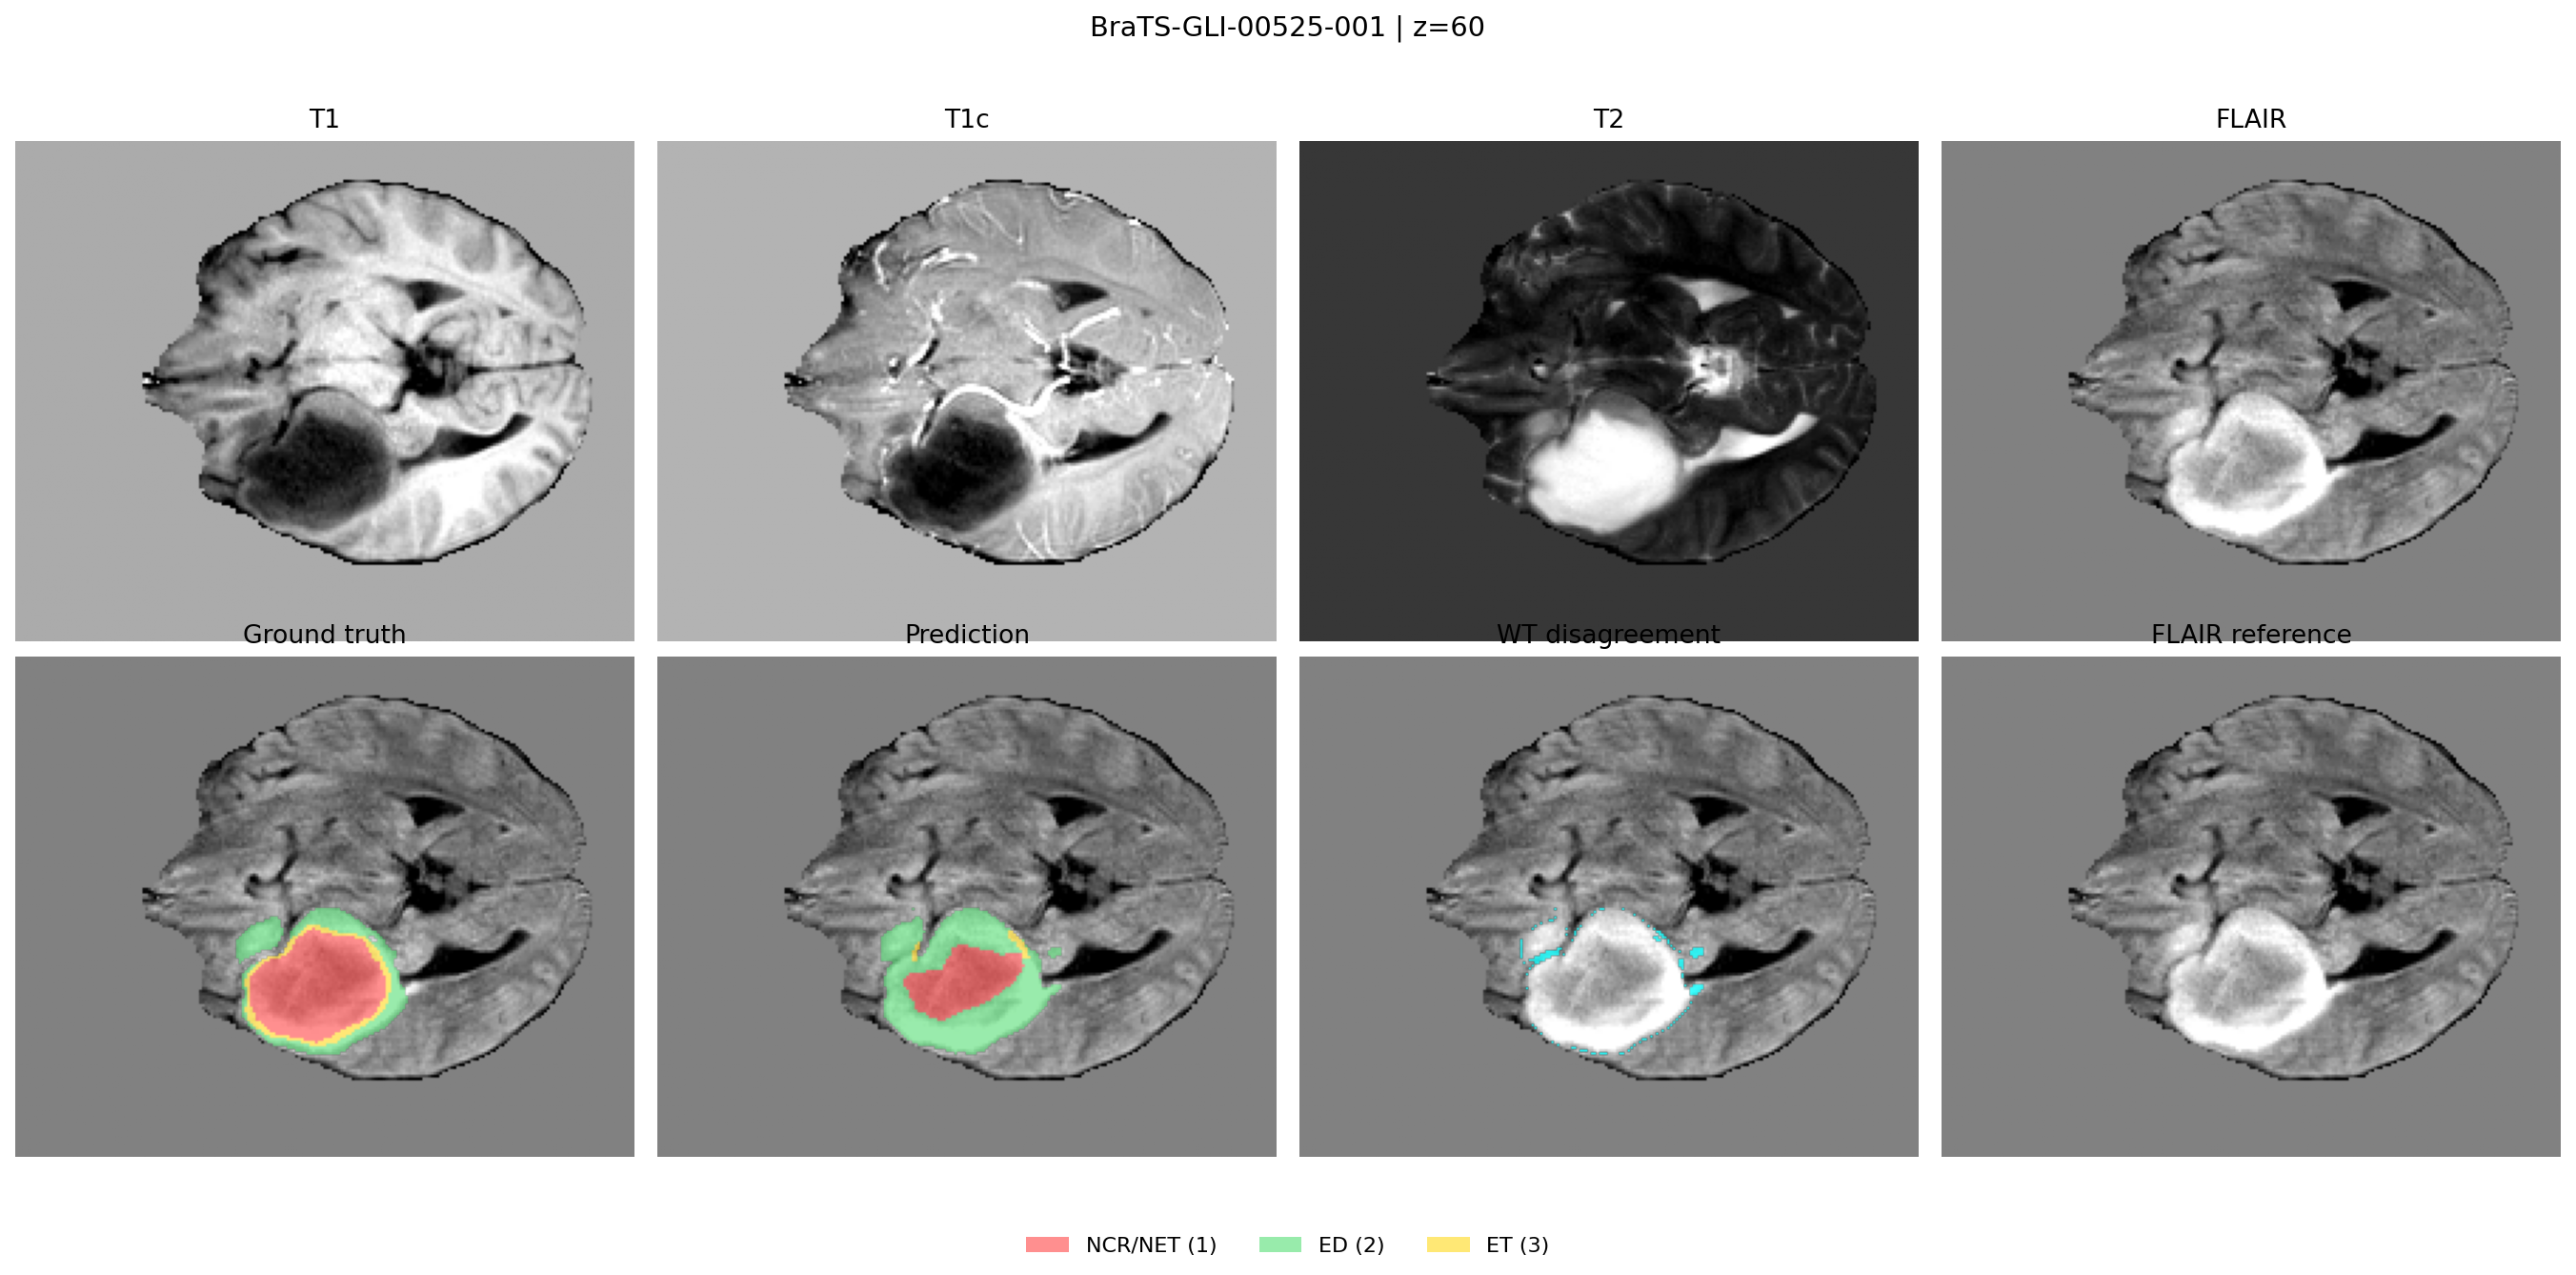
\includegraphics[width=0.48\linewidth]{../../outputs/taf_transbts_cluster_a3_finetune_resume_mmap/analysis/multimodal_badcase_figures_test/BraTS-GLI-00525-001.png}
\hfill
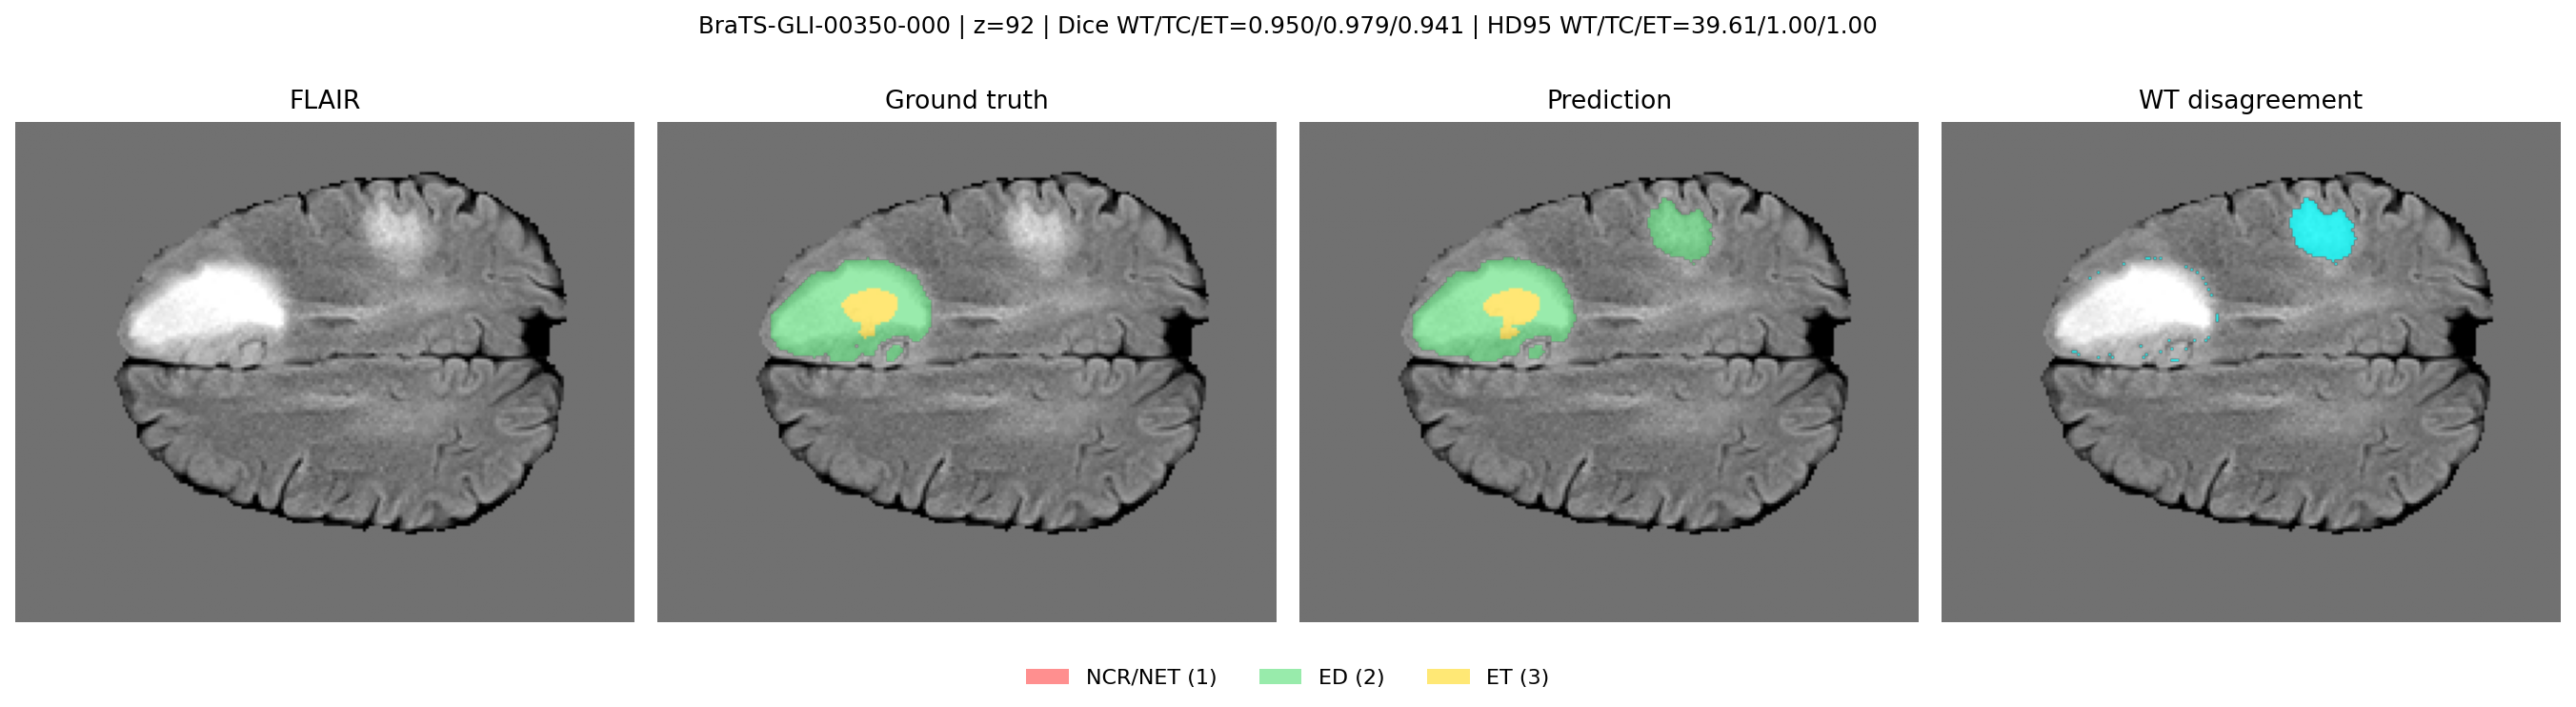
\includegraphics[width=0.48\linewidth]{../../outputs/taf_transbts_cluster_a3_finetune_resume_mmap/analysis/worst_case_figures_test/BraTS-GLI-00350-000.png}
\caption{左：WT Dice 很高但 ET rim 漏分，说明 WT 不能代表全部临床区域。右：Mean Dice 可达 0.9564，但 WT HD95 为 39.61，说明 Dice 会掩盖远端边界错误。}
\end{figure}

相对 TransBTS baseline，staged TAF A3 在 82/127 个病例上提升 Mean Dice。提升最大的病例包括 BraTS-GLI-00525-000（+0.189）、BraTS-GLI-00321-000（+0.181）、BraTS-GLI-00116-000（+0.157）、BraTS-GLI-00113-000（+0.128）和 BraTS-GLI-00485-000（+0.068）。后续报告可补充这些 improved cases 的可视化图，以展示 TAF 对 TC/ET 的修复效果。\\
\todo{建议从 paired case metrics 中挑选 BraTS-GLI-00525-000 或 BraTS-GLI-00321-000，生成 baseline-vs-TAF 对比图并复制到 \texttt{task3/pre/fig/case/}。}

\section{讨论：Task 2 与 Task 3 的差异}

当前最强 Task 3 模型 Fresh TAF-TransBTS A3 的 Mean Dice 为 0.9014，低于 Task 2 四模态二维 U-Net 的 0.9158，也低于 Task 2 精选四模态后续改进中的三模态 Dice 0.9295。这个差距反映出二维切片模型与三维 full-volume 模型在训练样本、输入视野和评估方式上的差异。

首先，二维模型拥有更多训练样本。Task 2 将三维体切成大量 axial slices，模型每个 epoch 接触到的样本数量远大于三维 patch 训练。二维模型还能看到完整 $177\times219$ axial plane，而三维模型训练时主要看到 $96^3$ patch。三维上下文提供了切片间连续性，同时带来了更高的优化难度和更强的类别不平衡。

其次，Task 2 的最优三模态模型属于后续模态选择改进。公平讨论四模态输入时，Task 2 四模态模型的 Mean Dice 为 0.9158，HD95 Mean 为 4.1394。Task 3 大多数正式模型保留四模态输入，并通过 attention 学习模态权重。现有结果显示，attention 可以缓解模态贡献差异，但还不能完全替代显式模态选择；TAF 三模态消融仍需要单独验证。

第三，HD95 揭示了 Dice 之外的风险。二维四模态模型的 HD95 Mean 为 4.1394，3D U-Net dual-attention 的 HD95 Mean 为 4.1125，Fresh A3 在 WT/TC 上相对 Fresh TransBTS 明显改善，但 ET HD95 仍有代价。这个现象与 badcase 分析一致：细小增强区域、薄 rim、远端假阳性组件会显著影响边界指标。Task 3 的价值在于把这些问题显式暴露出来，并用病例级分析指导下一步设计。

最后，full-volume training 更差的结果提示，扩大视野并不能单独解决问题。随机 patch 训练承担了数据增强和肿瘤区域重采样作用；后续优化更应关注模态选择/融合、小区域损失、组件后处理和推理阶段的边界稳定性。

\section{后续改进方向}

基于 HD95 和 badcase 分析，后续应优先做有针对性的验证，减少缺少诊断目的的模型堆叠：
\begin{itemize}
  \item 在 validation split 上验证 connected-component post-processing，重点减少小的远端 WT false positives，并同时观察 Dice 与 HD95；
  \item 在 sliding-window inference 中加入 Gaussian center weighting，降低 patch 边界伪影和碎片化；
  \item 对 TC/ET under-segmentation 做窄范围 loss ablation，例如适度提高 TC/ET 权重，或加入 boundary/surface loss；
  \item 对 Task 2 二维模型输出进行更细的病例级对照，特别比较四模态 2D、三模态 2D、Fresh A3 在相同病例上的 HD95 tail cases；
  \item 进行三模态 TAF 或三模态 3D U-Net 消融，检验 Task 2 中 selected modalities 的优势是否能迁移到三维模型；
  \item 尝试 2.5D 输入，作为二维样本效率与三维上下文之间的折中。
\end{itemize}

\section{结论}

本阶段的实验链条给出一个逐步收敛的结论。直接将 Task 2 的二维 U-Net 改为三维后，Mean Dice 停留在 0.8950 左右；TransBTS 通过 Transformer bottleneck 小幅提升 TC/ET；MSA、RAM/RAMS 和 RSF 依次验证了输入注意力、区域导向融合和区域监督特征融合的收益与风险。RSF 的远端假阳性和 RAM 的 WT 完全漏检病例促使最终方案转向 softmax-controlled fusion。

在同协议 fresh control 下，TAF-TransBTS A3 将 Mean Dice 从 Fresh TransBTS 的 0.8979 提升到 0.9014，并将 WT HD95 从 12.40 降到 5.71，TC HD95 从 3.06 降到 2.94。与 Task 2 四模态二维模型相比，TAF 的 Dice 仍有差距；与 Task 3 三维基线相比，它验证了受控多模态融合的价值。badcase 分析进一步指出，ET 小区域边界、薄 enhancing rim、低对比 diffuse WT 和远端假阳性是下一阶段更值得优化的方向。

\end{document}
